\documentclass[a4paper,11pt]{report}
\usepackage{a4wide}
\usepackage[frenchb]{babel}
\usepackage[utf8]{inputenc}
\usepackage[T1]{fontenc}
\usepackage{geometry}
\usepackage{graphicx}
\usepackage{fancybox}
\usepackage[pdftex]{hyperref} %Liens dans table de matieres
\usepackage{fancyhdr}
\usepackage{geometry}
\usepackage{url}
\usepackage{multicol}

\usepackage{pstricks}

%\geometry{scale=0.75, nohead}


\newcommand*{\enConstruction}[1]{
	\vspace*{.1cm}
	\doublebox{
	    \begin{minipage}{.9\linewidth}
	      --- #1 \\ 
	    \end{minipage}
	}
}

\newcommand*{\precision}[1]{
	\vspace*{.1cm}
	\fbox{
		\begin{minipage}{.9\linewidth}
			#1 
		\end{minipage}
  	}\\
}

% Title Page
\title{
	
\includegraphics[scale=.2]{logofds.eps}\\
	\vspace*{1cm}
	TER FMIN200 \\ 
	-- \\
	Développement d'un jeu de type Bomberman en réseau sous Android et iOS
}

\author{BONVILA Olivier \and COUSEIN Kilian \and PITIOT Ludovic \and TARDIEU Benjamin}

\date{}

\begin{document}
\maketitle

\thanks{

  Nous tenons à remercier 

}


\tableofcontents

\chapter{Introduction}

	Nous sommes amenés, dans le cadre de notre première annéee en master informatique à la faculté des Sciences de Montpellier, à travailler sur l’élaboration complète d’un projet, de son analyse à la conception puis à sa programmation. Tout au long de ce deuxième semestre, le projet nous per-met de comprendre quelles sont les phases de développement d’un projet et comment celui-ci doit être conduit. Nous pouvons par ailleurs mesurer notre capacité à réagir face à des problèmes en nous impliquant dans ce projet. Le projet que nous avons choisi est de réaliser sur deux système d'exploitation\footnote{Le système d'exploitation est l'ensemble de programmes central d'un appareil informatique qui sert d'interface entre le matériel et les logiciels applicatifs.} de téléphone différents un jeu de type Bomberman.

Ce projet nous permet de mettre en application l'enseignement que nous avons acquis tout au long de ce semestre. Ce dernier étant spécialisé pour chaque étudiant, il nous a permis de travailler en collaboration avec des personnes au capacités différentes et d'ainsi mettre nos connaissances en commun. Mais il permet aussi de ce faire une idée du travail demandé dans le monde des entreprises et d'ainsi nous préparer à notre stage que nous devrons réaliser l'an prochain.

Afin de comprendre la démarche que nous avons utilisée pour mener ce projet à son terme, notre rapport se compose de trois grandes parties : 

Tout d'abord, dans une première partie nous présentons le cadre général de notre projet, c'est-à-dire le groupe de projet, les outils de developpement ainsi que la manière dont nous nous sommes organisé pour mettre à bien le developpement de ce dernier. Ensuite dans une seconde partie, nous présenterons le travail d'analyse que nous avons effectué pour pouvoir ensuite, dans une troisième partie, expliquer le developpement du projet.

\chapter{Présentation}

	\begin{itemize}
		\item{Nous + Tuteur}
	\end{itemize}

	En tant que première année de master, nous avons dû développer un projet tout au long de ce semestre. Chaque année une liste de projets est présentée aux étudiants. Tous les étudiants doivent former des groupes pour développer l'un des projets choisi. Puis ces derniers sont associés à un tuteur. Etant donné que nous voulions développer notre propre projet, nous avons formé un groupe de quatre personnes : Olivier BONVILA, Kilian COUSEIN, Ludovic PITIOT et Benjamin TARDIEU. Ensuite,nous avons créé un sujet. Pour pouvoir valider notre sujet, nous avons dû trouver un tuteur voulant bien s'occuper de notre tutelle. Mr Laurent Deruelle a gentiment accepté de s'occuper de notre groupe, mais pour que ce dernier soit entièrement validé, des modifications du sujet ont été nécessaires.

\section{Projet}	
	
 Etant donné que nous voulions principalement créer une application IPhone, nous avons demandé à developper notre propre projet. Un jeu de type bomberman. Mais ce dernier a du subir des modifications pour être approuvé. Nous avons donc du developper le jeu sous IPhone et sous Android. Le but étant de comparé la différence de developpement entre les deux types de telephone et de developper des fonctionnalités en rapport avec les parcours d'enseignement que nous avons choisi ce semestre.\\
	
Un jeu de type bomerman est une jeu d'action dont le but est simple. Le joueur incarne un poseur de bombe et ce dernier doit faire exploser ses ennemis pour pouvoir gagner la partie. A ceci s'ajoute toute une liste de bonus et malus permettant de complexifier le jeu et de le rendre plus amusant.\\
	
Pour pouvoir rapprocher le developpement de cette application à notre parcours d'enseignement. Nous avons choisi de developper un mode solitaire qui permettra de jouer contre une ou plusieur intelligence artificelle qui est en rapport avec le cursus I2A\footnote{Ingéniererie de l'Inteligence Articielle} qui nous est enseigné. Ensuite pour ce qui est du parcours CASAR \footnote{Combinatoire, Algorithmique, Sécurité et Administration Réseau}, nous avons décidé de développer un mode multijoueur qui permettra à plusieurs joueurs connectés en WI-FI\footnote{Wi-Fi est un ensemble de protocoles de communication sans fil qui permet de relier sans fil plusieurs appareils informatiques au sein d'un réseau informatique afin de permettre la transmission de données entre eux.} de jouer en réseau grâce à un serveur qui combinera un serveur d'application et un serveur web. Puis pour ce qui est du parcours DIWEB \footnote{Données, Interaction et Web}, la partie serveur permettra de palier a l'enseignement de ce dernier parcours.
	
	

		

	
\section{Histoire du jeu}
	
\subsection{Histoire}

Le Bomberman est un jeu culte des années 80. Il a été conçu par l'éditeur japonais \href{http://www.hudsonsoft.net/}{Hudson Soft}. Sa silhouette, reconnaissable parmi toutes, est celle d'un poseur de bombes muni d'un casque avec des membres blancs et un corps bleu. Cependant, à la sortie du premier Bomberman en 1983 sur \gls{msx}, notre héros n'arborait pas cette apparence puisqu'il s'agissait en fait d'un ennemi issu de \gls{lode runner}. Ce n'est qu'en 1985 que l'aspect de Bomberman tel que nous le connaissons aujourd'hui est utilisé lors du portage sur \gls{nes}. C'est cette adaptation qui a réellement permis de faire connaitre le personnage en partie grâce à des mécaniques de jeu très simples.

Au fil du temps et des versions, le poseur de bombes gagne des pouvoirs de plus en plus grands. Ainsi, dans le premier épisode, le personnage ne sait que poser des bombes. Les bonus du jeu se limitent aux bombes, aux flammes et aux bottes permettant respectivement d'augmenter le nombre de bombes que l'on peut porter, la porté des explosions et la vitesse de déplacement. Dans les versions suivantes le personnage peut, après avoir trouvé les bonus correspondants, lancer des bombes ou les pousser, traverser les murs, etc. Certaines versions ont vu apparaitre des montures apportant de nouveaux pouvoirs et modes de déplacement.


\subsection{Principe}
Pour gagner, il faut détruire ses ennemis à l'aide de bombes et obtenir des bonus ou malus qui permettent d'augmenter ou diminuer ses chances de gagner. La maniabilité, le rythme effréné et la possibilité de s’affronter à quatre joueurs ont grandement contribués à sa popularité (dix millions d’exemplaires vendus depuis sa création). Sa simplicité, aussi bien dans le gameplay que dans les graphismes, semble être l’élément moteur de son succès puisque toutes les tentatives de suites, augmentant le nombre de bonus ou passant à la 3D, ont été boudées par le public. L’absence d’évolution du concept n’empêche aucunement à ce jeu d’être l’un des plus addictif du genre, et à son personnage de connaître une immense popularité. 

\section{Plate-formes de développement}
	\subsection{Android}
	\begin{itemize}
		\item{De qui ?}
		\item{Langage}
		\item{PC}
		\item{SDK - (le contenu)}
	\end{itemize}

\subsection{iOS}
	\begin{itemize}
		\item{De qui ?}
		\item{Langage}
		\item{Mac}
		\item{SDK - (le contenu)}
	\end{itemize}

	
	
\chapter{Analyse}
	\begin{itemize}
		\item{Introduction}
	\end{itemize}
	
	\section{Cahier des charges}
	\subsection{Menus}
		
	Les menus se doivent d'être clairs et de rendre l'utilisation de
	l'application aisée. Il s'agit d'un jeu ne demandant aucune compétence
	particulière. Il va donc toucher un public large et doit pouvoir convenir à
	tout utilisateur. Cela passe d'abord par une navigation intuitive dans les
	menus.
		
\subsection{Jeu}
		
	Le jeu est la partie la plus importante du projet. 
	Il se decompose en trois éléments : le model, la vue et le controlleur. 
	Le modèle est composé du moteur physique, du moteur de rendu ainsi que de la
	hierarchie de classes permettant de representer l'ensemble des objets du jeu. 
	La vue quant à elle est composée d'objets graphiques simples (bouttons, images, ... ) 
	et d'une partie reprèsentant le jeu. Elle se doit d'être ergonomique et de permettre
	à l'utilisateur de pouvoir jouer très simplement. Le controlleur fait
	le lien entre les actions de l'utilisateur sur le modèle. Cette décomposition aura
	l'avantage de pouvoir modifier facilement le modèle et/ou la vue.
		
	L'application doit aussi pouvoir changer de langue, avec comme langues initiales le francais et l'anglais.
	Elle doit permettre à l'utilisateur de jouer à des parties solitaires ou multijoueur. 
	Ce dernier possèdera un compte hors ligne et en ligne.		
	Le premier servira à personnaliser son profil comme par exemple pour modifier
	la couleur du joueur, changer son pseudo ou encore à enregistrer les informations
	et les preferences de connexion sur une base de données locale,
	mais également les scores du joueurs (nombre de parties gagnées ou perdus).
	
	Dans le jeu l'utilisateur peut créer différents comptes hors lignes en cas de partage du télephone
	avec un ami ou un membre de sa famille, pour pouvoir garder en mémoire ses scores et ses préferences.		
	Le compte en ligne quant à lui servira seulement à établir une connexion avec le serveur distant pour pouvoir jouer en multijoueur.		
	Un menu d'aide doit apparaitre afin d'aider le joueur à comprendre le but du jeu et comment jouer. 
	Ce dernier est simple et très explicite étant donné la large tranche d'âge des utilisateurs que vise cette application.		
	Ensuite un éditeur de carte permettra aux utilisateurs de créer un large choix de cartes
	grâce à une multitude de différents objets qui les composeront. Ces dernieres pourront être seulement utilisées en mode solitaire.
	Pour les parties solitaires une intelligence artificielle avec trois niveaux de difficulté 
	devra permettre à un joueur débutant, intermédiaire ou confirmé de jouer comme bon lui semble pour pouvoir améliorer sa maniere de jouer.
	
\subsection{Serveur}
	
	Le serveur représente la partie réseau de notre projet et rend fonctionnel le jeu entre plusieurs téléphones via des parties multijoueur (qu'ils soient de type
	\gls{ios} ou \gls{android}). Autrement dit il servira d'hebergeur pour les parties et
	il se chargera de l'intéraction entre les joueurs, via leur mobile.
	
	Il devra être capable d'enregistrer des inscriptions de nouveaux joueurs, avec
	vérification afin qu'il n'y ait pas de doublon. Ces derniers seront inscrits dans 
	la base de données du serveur. Les joueurs devraient ainsi
	pouvoir se connecter en utilisant le couple nom d'utilisateur/mot de passe,
	préalablement choisi. Suite à cela les utilisateurs seront à même de lister
	les parties en cours, ils pourront choisir de créer des parties ou de les rejoindres.
	
\section{Modélisation}
	\label{Modelisation}
	\subsection{Général}
	Le fait de développer des applications \gls{ios} et \gls{android}, nous a imposé le choix du langage. En effet pour développer des applications \gls{iphone}, il faut utiliser le langage \gls{objective-c}, puis  pour les applications \gls{android} c'est le langage \gls{java} qui est utilisé. C'est deux langages ont une syntaxe complétement différente mais sont quand même très proche car ce sont des langages orientés objets. Grâce à cela nous avons pu mettre au point une modélisation générale de l'application que nous avons ensuite adapté à chaque langage.\\
			
	Nous avons décidé de développer en anglais car premièrement c'est la langue la plus utilisé dans le monde de la programmation et deuxièmement car la syntaxe des langages est toujours en anglais. Cela permettra à n'importe quel utilisateur de n'importe quelle nationalité de comprendre le code de l'application.\\
			
	La documentation des deux applications est également en anglais. Cette documentation permettra à tout utilisateur de comprendre le fonctionnement de l'application.
	Nous avons créé une documentation pour l'application \gls{iphone} et pour l'application \gls{android}. Chacune de ces documentations est au format \gls{html} et sera donc directement visible grâce à un navigateur Web.\\
			
	Pour ce qui est de la modélisation globale du projet, nous avons choisi de développer les deux applications selon le modèle \gls{mvc}. Ce dernier est une architecture et une méthode de conception qui organise l'\gls{ihm} d'une application logicielle. 
			
	Le modèle représente le comportement de l'application : traitements des données, interactions avec la base de données, etc. Il décrit et contient les données manipulées par l'application. Il assure la gestion de ces données et garantit leur intégrité.
			
	La vue correspond à l'interface avec laquelle l'utilisateur interagit. Sa première tâche est de présenter les résultats renvoyés par le modèle. Sa seconde tâche est de recevoir toutes les actions de l'utilisateur (clic de souris, sélection d'une entrée, boutons, etc).
			
	Le contrôleur prend en charge la gestion des événements de synchronisation pour mettre à jour la vue ou le modèle et les synchroniser. Il reçoit tous les événements de l'utilisateur et enclenche les actions à effectuer.
			
	Grâce à cette méthode de conception le code est décomposé en trois parties bien distinctes qui permettent la maintenance et l'amélioration du projet. Cela permet aussi de modifier chacune des trois parties sans avoir à modifier les deux autres. Cela permet par exemple de changer de vue et avoir des interfaces graphiques différentes.
			
\subsection{Menus}

	Au démarrage de l'application vous arrivez sur un menu d'accueil. Depuis
	celui-ci vous pourrez accéder à l'aide, à la liste des comptes locaux ou à la
	création d'un nouveau compte local.
	Les menus de l'application ont été réalisés pour que l'utilisateur puisse les utiliser de manière intuitive. Ils se divisent en quatre grandes sections.
		
	Vous avez tout d'abord la section de création de parties locales. Vous aurez
	accès à une liste de cartes ainsi qu'au réglage de difficulté des \glspl{bot}, leur
	nombre et le temps de jeu. Le type de partie sera une fonctionnalité à venir.
	Vous n'aurez plus qu'à créer la partie configurée.
		
	Dans la même catégorie se trouve la section des parties multijoueurs. En
	accédant à celle-ci vous allez pouvoir vous connecter à votre compte
	multijoueur, ou le créer s'il n'est pas déjà fait. Vous accèderez ensuite à la liste
	des parties multijoueurs, que vous pourrez rejoindre, ou choisir de créer la
	votre. Dans le menu création le principe est proche des parties locales.
		
	Suite à ces deux sections vient ensuite l'éditeur de cartes. C'est depuis ce
	menu que vous créerez une nouvelle map de jeu local ou éditerez l'une d'entre elles. Choisisez votre nom de carte et l'éditeur
	s'ouvrira ensuite à vous. Il vous sera possible, à la fin, d'enregistrer votre
	carte si vous désirez la conserver et l'utiliser comme carte de jeu.
		
	Et enfin vient le menu des options. Depuis ce dernier vous pourrez gérer vos
	préférences sytèmes telles que le volume ou la langue de
	l'application(anglais, français).
	Une sous-section de gestionnaire de profil est aussi présente. Une édition de vos comptes locaux, multijoueurs ou même
	vos paramètres de jeu comme la position du menu, sont modifiable depuis ce
	menu à onglets.
	
	\begin{figure}
		\label{activité}
		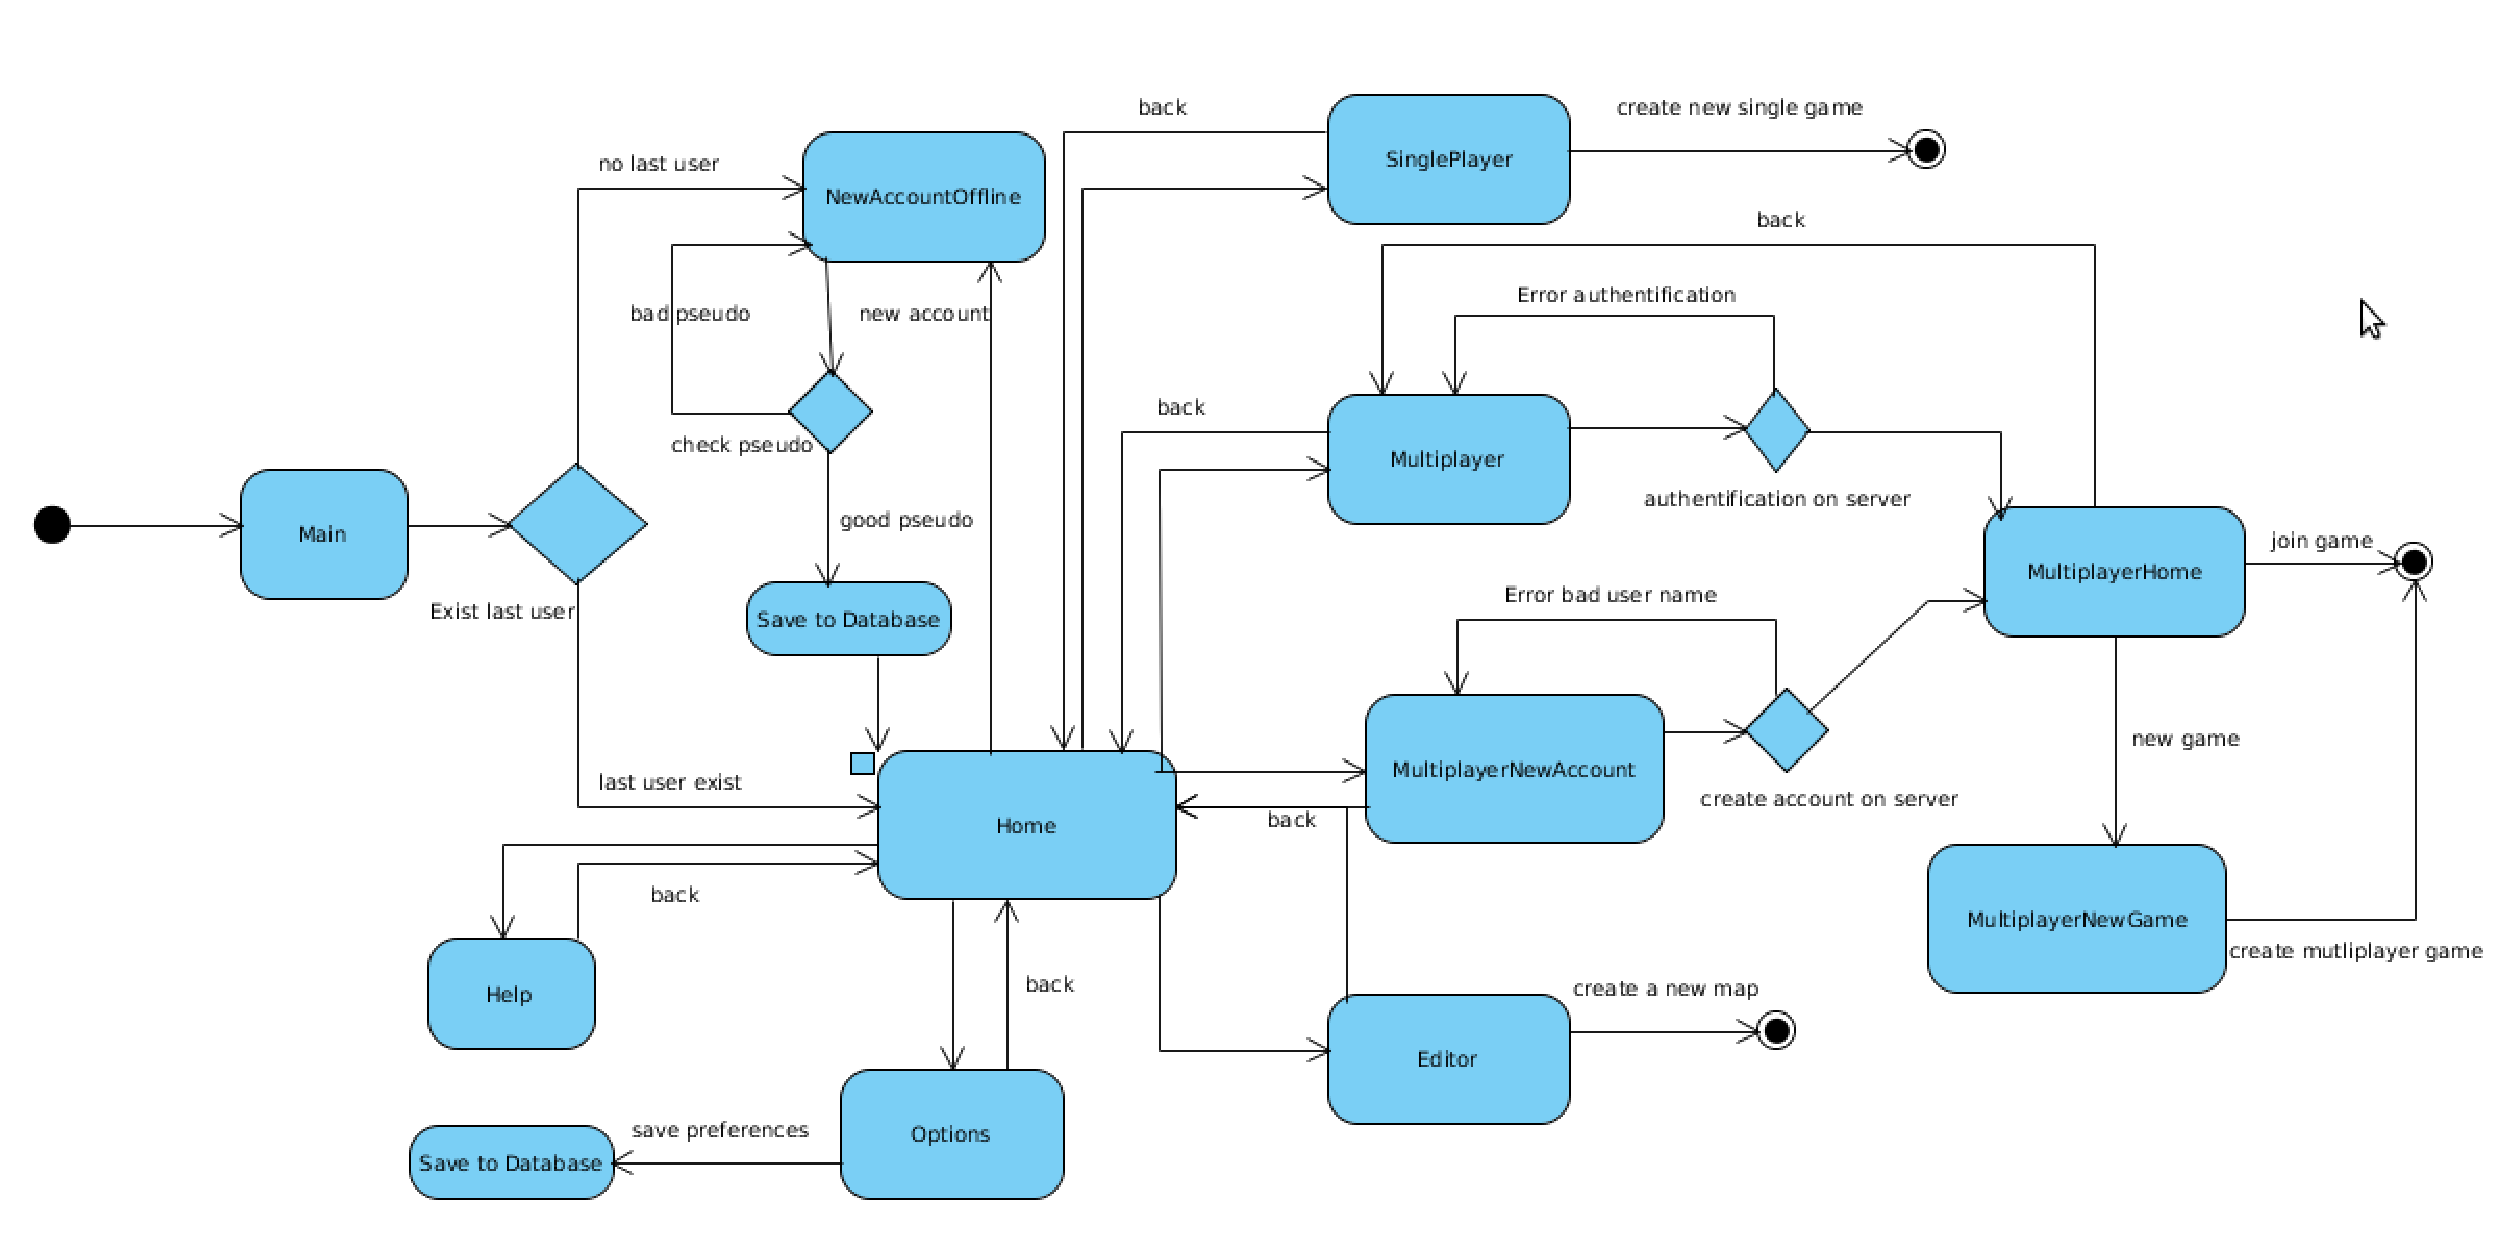
\includegraphics[width=23cm, angle=90]{Analyse/Img/diag_activity.eps}
		\caption{Diagramme d'activité}
	\end{figure}

	\paragraph{Base de données\\}
			
		Une base de données locale a elle aussi été conçue. Cette dernière a pour
		but de stocker plusieurs types de données.
				
		En effet dès lors qu'un compte local est créé sur le téléphone dans la
		table PlayerAccount, il est possible de conserver ses préférences de joueur
		tel que la couleur du joueur, le pseudonyme ou même ses paramètres de connexion multijoueur. 
		Vous pourrez créer autant de comptes locaux que vous désirez, et il
		sera possible possible d'éditer ou choisir son compte.
				
		L'application est par ailleur en mesure de conserver
		les valeurs sonores, la langue et même le dernier utilisateur de
		l'application, grâce à un son id qui est clé étrangère dans la table System(attribut lastUser).
				
		De plus l'application sera délivrée avec quelques cartes officielles, mais
		l'utilisateur aura libre droit de créer ses propres cartes de jeu via un
		éditeur. Elles seront alors stockées dans la table Map avec toujours une
		clé étrangère vers l'id de son créateur(owner). \\
		
		\newpage
				
		\begin{figure}
			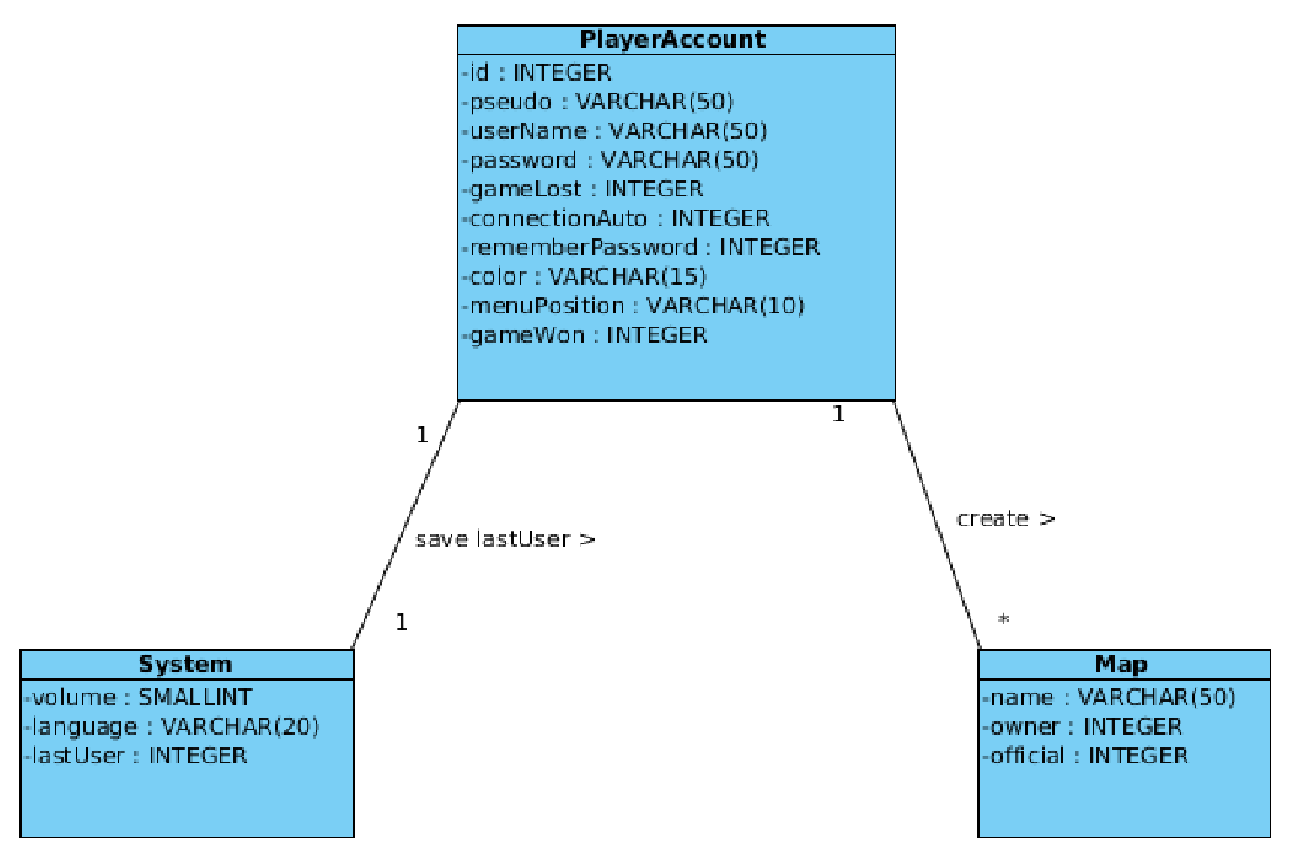
\includegraphics[width=11cm]{./Analyse/Img/menu_bdd.eps}
			\caption{Diagramme de classe Base de données}
		\end{figure}
		
		
		
						
	\paragraph{Scénarios}
	
	
\subsection{Editeur de carte}	

	L'éditeur de carte est une fonctionnalité qui va permettre à un utilisateur de créer facilement ses propres cartes pour ensuite y jouer dessus contre l'intéligence artificielle. Après avoir réfléchi sur toutes les fonctionnalités que l'éditeur de carte devait remplir, nous avons retenu celles-ci : permettre à l'utilisateur de créer une nouvelle carte, mais aussi de charger une ancienne carte précèdemment créée. Ensuite lui donner la possibilité de modifier le sol de la carte et aussi ajouter ou supprimer des blocs de la carte et enfin la dernière fonctionnalité que l'éditeur de carte implémente c'est de pouvoir placer les différents points de départ des joueurs sur la carte.
		
	Pour réaliser cette partie de l'application, nous avons utilisé le modèle de conception MVC pour diviser le code de l'éditeur de carte. Grâce a cette décomposition, le code est plus lisible et plus facile à réutiliser. 
			
	\subsubsection*{Modèle}
		La partie modèle va contenir toute les données de l'éditeur de carte. Les cartes sont les principales données qu'il va devoir manipuler. Pour cela nous avons décidé de la réprésenter sous la forme de deux matrices, la première représentant les objets du premier niveau (le sol) et la deusième la matrice du second niveau (les blocs, les points de départ des joueurs, etc).
			
			
	\subsubsection*{Vue}
		Ensuite, la vue représentera l'interface graphique de notre éditeur de carte. La principale difficulté pour réaliser l'interface graphique était de devoir rentrer toutes les informations nécessaires pour l'éditeur de carte dans un écran de type \gls{smartphone}. Après plusieurs prototypes d'interface, nous avons décide de séparer l'interface en trois parties. Tout d'abord la plus grande partie, l'affichage de la carte, qui comment étant la principale information à afficher, nous avons essayé de maximiser sa taille. Ensuite un menu à droite permettant au joueur de changer d'outil. Et la dernière partie affiche les différents éléments permettant de controler l'éditeur de carte. L'utilisateur aura juste à choisir l'outil qu'il veut placer sur la carte grâce au menu de droite et ensuite lui suffira d'appuier sur la carte pour placer un bloc dessus.
		
%		\begin{figure}
			\begin{center}
				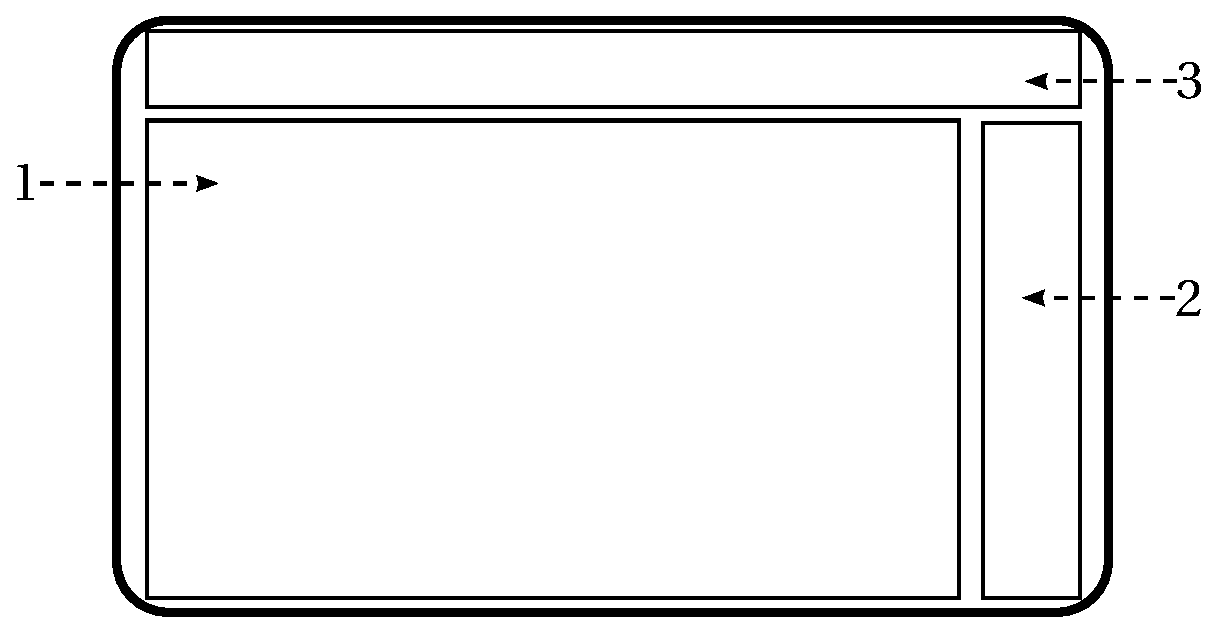
\includegraphics[width=11cm]{./Analyse/Img/14-Editeur_de_niveau.eps}
			\end{center} 
%		 	\caption{Poulpy est multicolore}
%		 	\label{Poulpy est multicolore}
%		\end{figure}
			
			
	\subsubsection*{Controleur}
		Pour finir le controleur aurra pour but de faire la liaison entre les données du modèle et de la vue. Chaque vue possède son controleur, et il y a un controleur gobal possédant les controleurs de chaque vue.
			

\subsection{Jeu}
	\subsubsection{Intelligence artificielle}
		Comme nous avons vu dans le cahier des charges, nous avons mis en place une integellence artificielle permettant à un joueur de jouer en solotaire.
	
		Tout d'abord nous avons du réfléchir à toutes les actions que les bots pourraient effectuer, lors d'une partie.
		
		
		L'intelligence artificielle dans notre jeu utilise des algorithmes de \gls{recherche_op}.
		
		Pour une meilleure expérience de jeu nous avons séparé l'intelligence artificielle en trois niveaux.
		
		$\,$
		
		\begin{itemize}
		  \item Facile
		  \item Moyenne
		  \item Difficile
		\end{itemize}
		
		$\,$
		
		Nous avons utilisé deux types d'algorithmes de \gls{recherche_op} basés sur le \gls{pathfinding}.
		
		\paragraph{Pathfinding}
		
			Le premier algorithme basé sur le parcours en largeur est utilisé quel que soit
			le niveau de l'intelligence artificelle choisie contrairement au second qui n'est utilisé
			que pour la difficulté moyenne et difficile.
		
		\subparagraph{Parcours en largeur\\}
		
			L'algorithme du parcours en largeur dans notre cas, consiste à partir d'un sommet S,
			lister d'abord tous les voisins de S pour ensuite les explorer un par un.
			Ici nous allons donc regarder toutes les cases autour de nous puis regarder
			tous leurs voisins et cela ainsi de suite jusqu'à trouver un point
			correspondant à nos attentes.
			
			Le contexte est le suivant, un \gls{bot} découvre qu'il est sur la trajectoire
			d'explosion d'une bombe est va donc fuir vers la case sûr la plus proche or
			il n'a aucune idée d'où elle se trouve.
			
			L'image suivante représentera la situation initiale :
			
			\begin{center}
				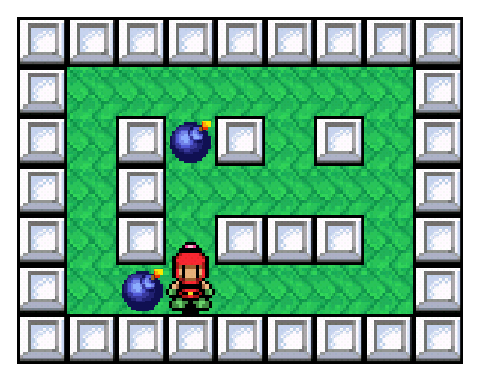
\includegraphics[width=8cm]{./Analyse/Img/largeur_0.eps}
			\end{center}
			
			Comme dit précédemment il n'y a que les murs ou les bombes que l'on ne peut
			pas traverser sinon tous les autres objets ou joueurs sont traversables.
			Nous considerons que les bombes ont ici un champs d'explosion en nombre de
			cases de 5.			
			
			Représentons la carte ci-dessus d'une façon plus parlante en remplacant les
			divers objets mis à par le joueur par des couleurs leur correspondant, à
			savoir :
			
			\begin{center}
				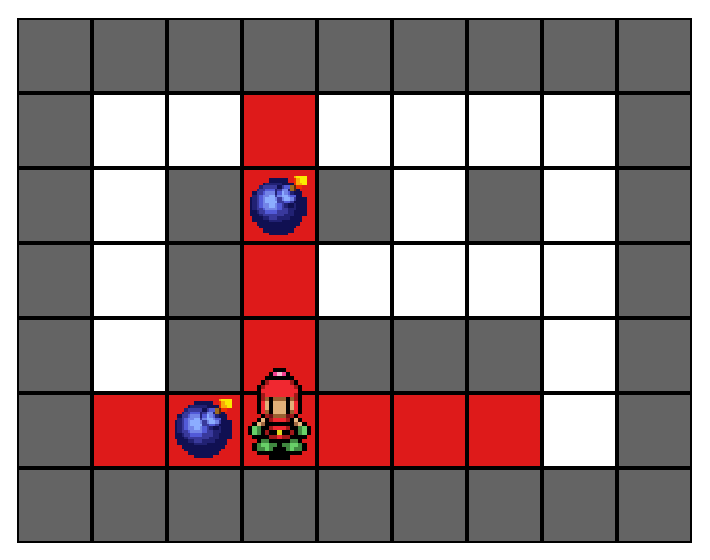
\includegraphics[width=8cm]{./Analyse/Img/largeur_1.eps}
			\end{center}
			
			Mettons nous à present à la place du \gls{bot}.
			
			Nous allons donner un poid aux cases que nous allons parcourir
			correspondant à la distance par rapport à la case initiale, ainsi qu'une
			direction qui correspondra à la direction initiale que le \gls{bot} devra empruter
			pour utiliser ce chemin, c'est à dire par exemple que tout chemin découvert
			dont l'origine est une case à droite de la notre aura comme direction droite.
			
			A partir d'une case donnée, nous ne regarderons que les voisines ayant un poids de 0
			car si leur poids est différent cela voudra dire que nous les avons déjà vu precedemment et bien évidemment,
			nous ignorerons les murs ainsi que les bombes.
			
			Nous avons changé la valeur des cases intraversables pour ne pas confondre avec le poids des cases visitées.			
			
			Appliquons l'algorithme de parcours en largeur aux cases voisines de la notre.
			
			
			\begin{center}
				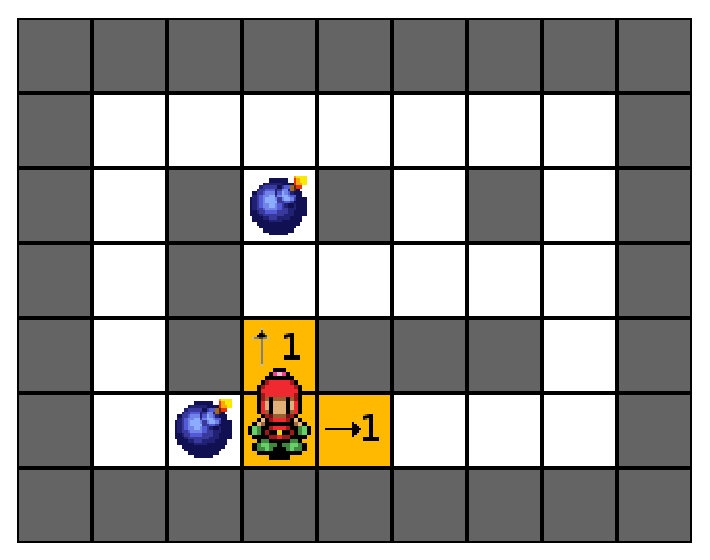
\includegraphics[width=8cm]{./Analyse/Img/largeur_2.eps}
			\end{center}
			
			
			Toutes les cases découvertes étant considérées comme dangereuses (voir le schéma précédent) nous continuons à appliquer l'\gls{algorithme} jusqu'à arriver à notre but.
			
			\begin{center}
				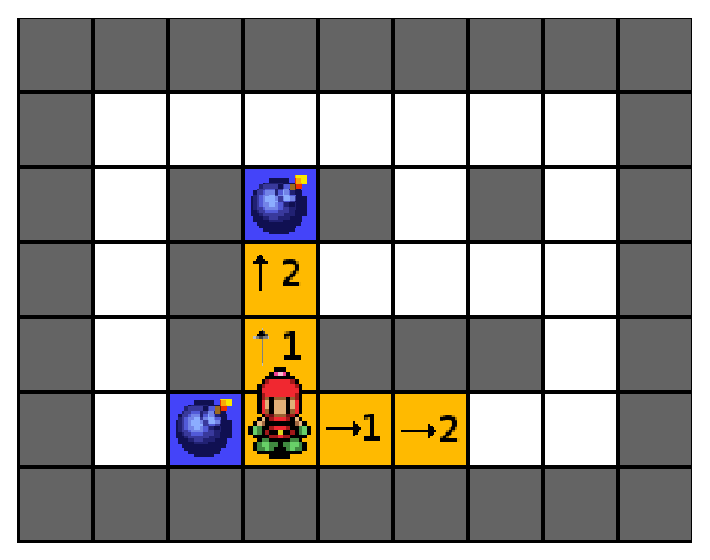
\includegraphics[width=8cm]{./Analyse/Img/largeur_3.eps}
				
				$\,$
				
				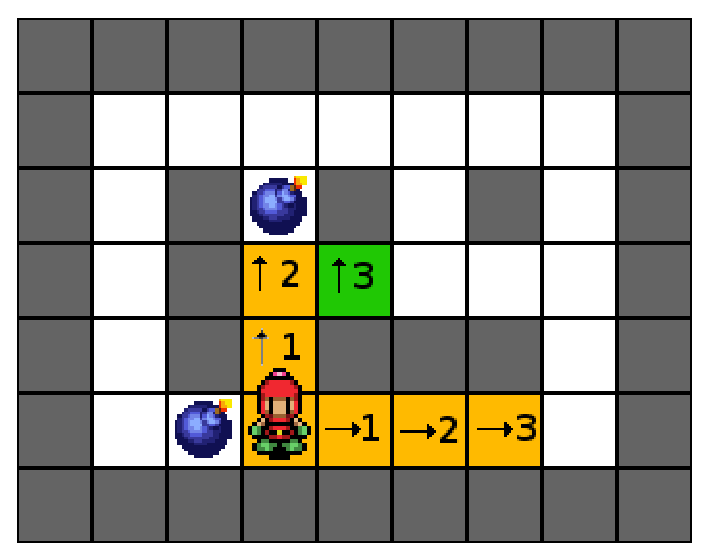
\includegraphics[width=8cm]{./Analyse/Img/largeur_4.eps}
			\end{center}
			
			Ici nous avons découvert une case non dangeureuse en $(13,6)$.
			
			Nous récupérons donc la direction enregistrée dans cette case et bougeons en fonction de celle-ci.
			
			Si plusieurs cases avaient été découvertes le choix aurait été arbitraire car elles auraient toutes été à la même distance.
			
			$\,$
			
		\subparagraph{A*\\}
		
			L'action la plus importante que l'intelligence artificielle doit savoir faire c'est de pouvoir se déplacer librement sur la carte en fonction des différents objets présents sur la carte et des actions effectuées par les autres joueurs.
		
			L'algorithme de recherche A* a pour but de rechercher un chemin
			dans un graphe entre un nœud initial et un nœud final tous deux préalablement
			définis. A* permet de trouver l'un des meilleurs (mais pas forcément le
			meilleur) chemins existant entre un point A et un point B (il retourne le premier chemin trouvé).
			
			La force de cet algorithme est le temps de calcul et l'exactitude des résultats, contrairement à Dijkstra qui lui fournit toujours le meilleur résultat (le plus court chemin entre deux points) mais dans un temps d'exécution beaucoup plus long que l'algorithme de A*.
			
			Sachant qu'il peut y avoir jusqu'à trois \glspl{bot} et que l'intelligence artificielle doit régulièrement recalculer son chemin en fonction des actions effectuées par les autres joueurs, nous avons donc choisi l'algorithme de A*.
		
			Maintenant que l'on sait quel algorithme utiliser pour rechercher un chemin dans un graphe, nous allons voir en détail comment marche l'algorithme de A*.
		
			Pour comprendre comment l'algorithme marche, nous allons nous aider d'un
			dessin représentent une carte avec un point A (départ) affiché en vert, un
			point B (arrivée) en rouge, et où les cases en bleu représentent les murs.
		
			\begin{center}
				\includegraphics[width=8cm]{./Analyse/Img/Grille.eps}
			\end{center}
		
			La premier chose que l'on peut observer, c'est que la carte est divisée en
			cases. Chaque case de la matrice représente un node qui peut être soit
			traversable, soit non traversable. Dans l'application, il n'y a que les murs
			ou les bombes que l'on ne peut pas traverser sinon tous les autres objets
			ou joueurs sont traversables. Le but de l'algorithme est donc de
			trouver un chemin entre A et B en évitant les murs.
			
		
			Durant le déroulement de l'algorithme, nous avons utilisé deux listes qui contiennent des cases de la carte.
			Il y a une liste dite \og listeOuverte \fg \, et l'autre \og listeFermée \fg.
			La listeOuvrete contient une liste de cases qui pourraient éventuellement faire partie du chemin, mais pas forcément, pour le moment elle sera vide.
			Plus précisément c'est une liste de cases que nous devons vérifier.
			Ensuite, au niveau de la listeFermée, elle contient toutes les cases que nous
			aurons déjà vérifiées, au début de l'excution, elle contient que le point de départ (B3).
			
		
			Commencons les explications du déroulement de l'algorithme.
			Tout d'abord, il faut savoir qu'un joueur peut se déplacer dans toutes les
			directions, donc nous allons ajouter toutes les cases adjacentes à la
			listeOuvert qui sont traversables, il y en a huit (A2, B2, C2, A3, C3, A4, B4, C4).
			
			
			Ce qui nous donne :
		
			\begin{center}
				\includegraphics[width=8cm]{./Analyse/Img/Grille2.eps}
			\end{center}
		
			Les carrés avec un contour rouge sont les carrés présents dans la
			listeOuverte et les carrés qui ont une couleur un peu plus foncée que les
			autres sont ceux qui se trouvent dans la listeFermée.
		
			Maintenant pour choisir la case par laquelle on doit passer, nous devons rajouter trois données \og F \fg , \og G \fg \, et \og H \fg:
			\begin{description}
				\item[G : ]{c'est le coût de mouvement pour aller de la case A à une case donnée sur la grille, en suivant le chemin généré jusqu'à cette dernière.}
				\item[H :]{c'est l'heuristique, c'est à dire le coût estimé pour allé du point courant à l'arrivé. Comme nous ne connaissons pas vraiment la distance qu'il nous reste à parcourir, car toutes sortes d'obstacle peuvent se trouver sur notre chemin (objet non traversable). Donc nous allons devoir l'approximer grâce à une fonction, pour la calculer nous avons choisi d'utiliser l'heuristique de Manhattan, qui consiste à compter le nombre de bloc (à vol d'oiseau et sans prendre les diagonales) qui lui reste à parcourir.}
				\item[F :]{c'est G + H}
			\end{description} 
		
			Chaque case de la listeOuverte ou de la listeFermée vont devoir possèder toutes ces données, plus les coordonnées de leur père, c'est à dire les coordonnées de la case qui vient de les ajouter dans la la listeOuverte. Pour calculer G, nous allons assigner un coût de 10 pour chaque déplacement horizontal ou vertical, et un coût de 14 pour un mouvement en diagonale. Nous utilisons ces données car la distance nécessaire pour se déplacer est la racine carrée de 2, ou approximativement 1.41 fois le coût d'un déplacement vertical ou horizontal. Nous utiliserons donc 10 et 14 pour des raisons de simplification. Par conséquent, nous allons multiplier par 10 le coût H pour qu'il soit cohérent par rapport à G.
	
			Donc maintenant, nous devons avoir cette matrice :
			\begin{center}
				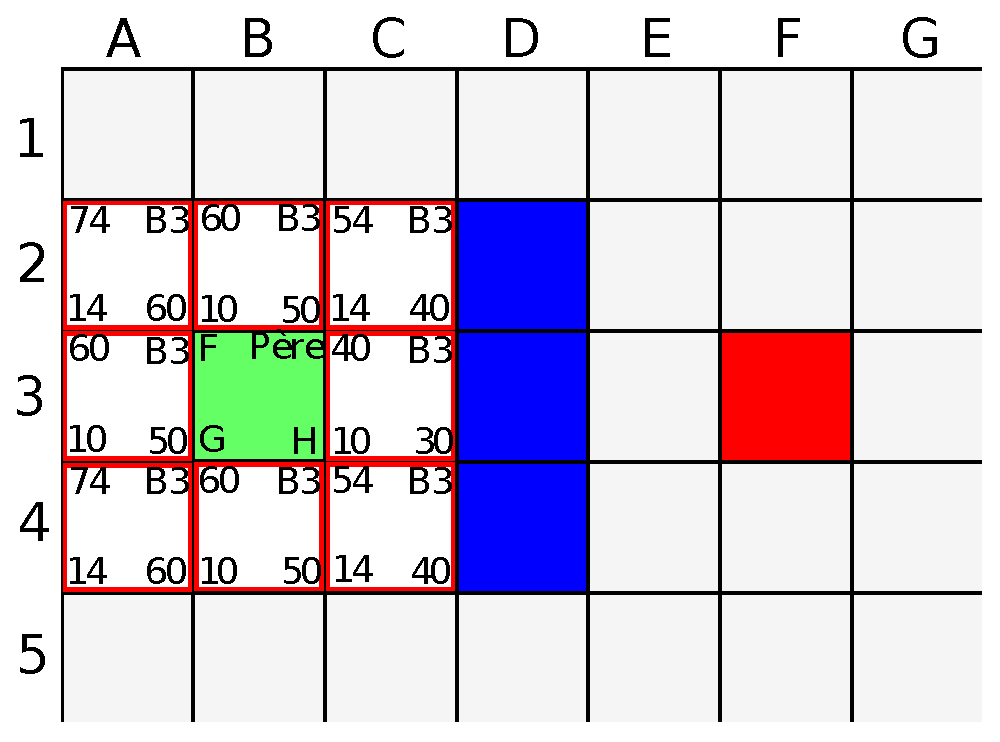
\includegraphics[width=8cm]{./Analyse/Img/Grille3.eps}
			\end{center}
		
			Après avoir ajouté toutes les cases adjacentes à la case courant, il suffit de prendre la case qui a le plus petit coût F et ensuite de la rajouter dans la listeFermée et de la supprimer de la listeOuverte. Nous obtenons donc :
			\begin{center}
				\includegraphics[width=8cm]{./Analyse/Img/Grille4.eps}
			\end{center}
		
			Ensuite on regarde toutes les cases adjacentes à la dernière case ajoutée dans la listeFermée. Si elles se trouvent déjà dans la listeOuverte, on vérifit que leurs coût soient inférieur au coût de la case correspondante déjà dans la listeOuverte, si oui alors on la remplace sinon on ne fait rien.
		
			Pour finir on répète cette opération jusqu'on arrive à la case d'arrivée, nous obtenons ça :
			\begin{center}
				\includegraphics[width=8cm]{./Analyse/Img/Grille5.eps}
			\end{center}
		
			Pour finir, il nous suffit juste de récupérer la case d'arrivée et de regarder son père, puis de repéter cette opération avec la case obtenu jusqu'à arriver à la case de dépard. Grâce à ça nous obtenons cette dernière étape de l'algorithme :
			\begin{center}
				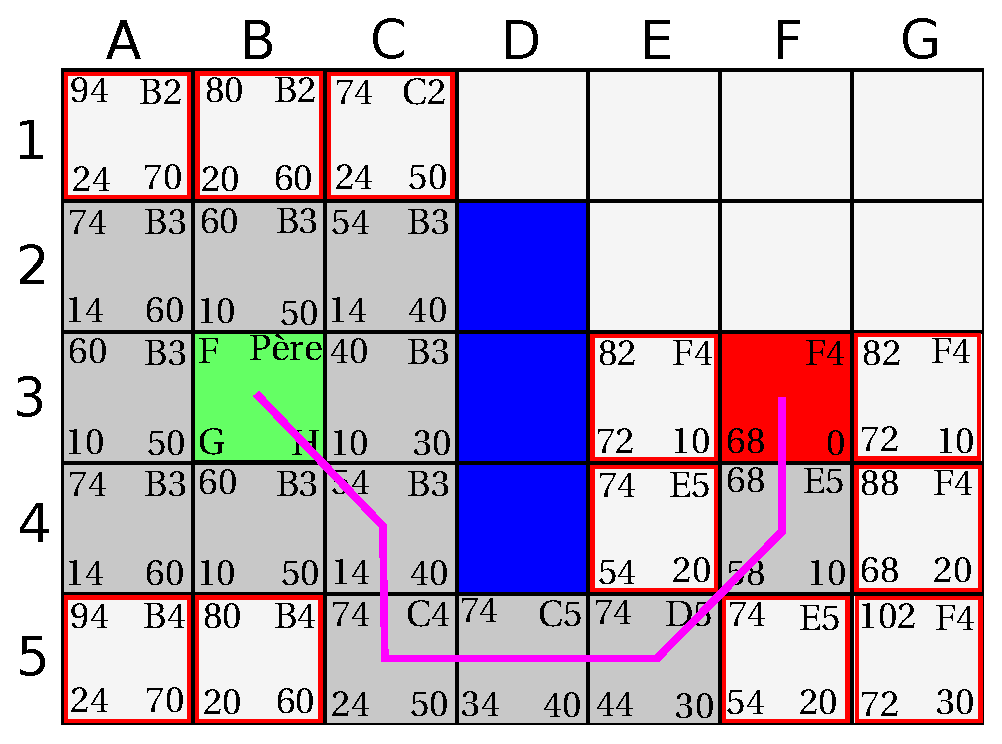
\includegraphics[width=8cm]{./Analyse/Img/Grille6.eps}
			\end{center}
		
			Comme nous pouvons levoir sur le schéma precedent, le chemin qu'a trouvé l'algorithme de A* est le suivant : $ B3 \rightarrow C4 \rightarrow C5 \rightarrow D5 \rightarrow E5 \rightarrow F4 \rightarrow F3 $. L'algorithme aurait pu d'autre chemin équivalent à celui-ci mais le principe de cette algorithme c'est de renvoyer le permier chemin qu'il trouve.
		
	\begin{itemize}
		\item{Diagramme classe}
	\end{itemize}
	
	Comme vue dans le cahier des charges, l'application est divisée en trois grandes parties: le modèle, la vue et le contrôlleur.
	
	\subsubsection{Modèle}
	
	Le modèle constitue la \textit{base} de notre projet. C'est sur celui-ci que nous avons construit le reste de l'application. Nous avons modélisé celui-ci de manière à ce qu'il soit clair et simple. Ce dernier ce décompose en trois sous-partie: la partie hierarchie des objets, la partie moteur puis la partie éditeur de carte.\\
	
	\paragraph{Hierarchie des objets \\}
	
	Pour concevoir la hierarchie des objets, il a fallu tout d'abord dinstinguer la totalité des objets qui seraient disponible dans le jeu ainsi que leurs différences et leur point communs.  Nous avons donc distingué quatre grands types d'objets: les objets destructibles, les objets indestructibles, les objet animés ainsi que les objets inanimés. En sachant que les objets pouvaient être destructibles-animés, destructible-inanimés, indestructible-animés ou indestructible-inanimés. Nous avons choisi que tout objet serait considéré comme un objet animé pour éviter des soucis de modélisation. Ainsi les objets possèderont tous une sequence d'animation d'images qui sera dessiné a l'écran. Cette derniere sera répété dans le cas d'une animation qui se répété et qui comporte plusieurs images, sinon si elle possède simplement qu'une seule image, seule cette image sera dessiné a l'écran. Nous avons ensuite dinstingué une multitude de point communs entre les différents objets dont voici le nom de l'attribut et leur utilité : 
	
	\begin{description}
		\item [\textit{position}]{indique la position en pixel de l'objet sur l'écran}
		\item [\textit{nom}]{indique le nom de l'objet}
		\item [\textit{hit}]{est à 1 si l'objet peut être touché par une explosion (0, sinon)}
		\item [\textit{level}]{est à 1 si l'objet est animés (0,sinon)}
		\item [\textit{fireWall}]{est à 1 si l'objet ne laisse pas passer les flammes des explosions (0,sinon)}
		\item [\textit{damages}]{indique si l'objet peut infliger des domages}
		\item [\textit{idle}]{est une image qui représente l'objet en général}
		\item [\textit{animates}]{est une table de hachage contenant l'ensemble des images composant la sequence d'animation de l'objet (vide si inanimés)}
		\item [\textit{destroy}]{est une table de hachage contenant l'ensemble des images composant la sequence d'animation de destruction de l'objet (vide si indestructible)}
		\item [\textit{currentFrame}]{permet de connaitre le numéro de l'image courante de la sequence d'animation en cours d'affichage}
	\end{description}

	Nous avons donc décider de concevoir une classe "Object"  pour modéliser toutes ces propriétés que les objets ont en commun. Cette classe sera abstraite car tout objet est destructible ou indestructible et cela sera décris dans des classes plus spécialisés.
	
	 Ensuite nous avons pensé a créer deux autres classes: "Destructible" et "Undestructible" pour les objets destructible et indestructible. Ces deux classes héritent de "Object" car elles sont des objets. Ce qui différencie ces deux classes est le champ \textit{life} qui permet de savoir combien de fois l'objet doit etre touché par une bombe avant d'être detruit.
	
	Nous avons ensuite dinstingué deux autres types d"objets encore plus spécifique: Les joueurs et les bombes. Ces derniers sont des objets destructibles puisqu'il ne dure pas toute la partie selon le mode de jeu.
	
	Les bombes possèdent deuxnouveaux attributs qui les différentie des autres objets: 
	\begin{description}
		\item [\textit{type}]{permet de connaitre le type de bombe}
		\item [\textit{owner}]{permet de connaitre le joueur qui a posé la bombe}
	\end{description}
	
	Quand à la classe joueur celle-ci possède encore d'autres attributs: 
	\begin{description}
		\item [\textit{color}]{permet d'afficher à l'écran le joueur avec sa bonne couleur}
		\item [\textit{bombsTypes}]{permet de connaitre le type de bombe qu'il peut poser}
		\item [\textit{powerExplosion}]{permet de connaitre la porté d'explosion de ses bombes}
		\item [\textit{timeExplosion}]{permet de connaitre le temps d'explosion des bombes}
		\item [\textit{speed}]{permet de connaitre la vitesse du joueur}
		\item [\textit{shield}]{permet de connaitre la valeur du bouclier}
		\item [\textit{bombNumbers}]{permet de connaitre le nombre maximum de bombes que le joueur peut poser}
		\item [\textit{isTouched}]{permet de savoir si le joueur viens d'être touché}
		\item [\textit{isKilled}]{permet de savoir si le joueur est mort}
		\item [\textit{isInvincible}]{permet de savoir si le joueur est invincible}
	\end{description}
	
	Cette hierarchie de classe nous permettra donc de modéliser l'ensemble des objets que le jeu pourra afficher.
	
	
	
	\paragraph{Moteur\\}
	
	Pour ce qui est du moteur. Celui-ci est représenté par une classe "Engine". Cette classe va contenir l'ensemble des méthodes qui vont permettre d'établir les collisions. C'est aussi cette classe qui s'occuppe de mettre à jour les bombes ainsi que l'IA du jeu. 
	Une instance d'un moteur est associée à une partie dont le nom de classe est "Game". Cette classe "Game" est abstraite et représente une partie avec toutes les options qu'elle contient. C'est à dire qu'elle possède des attributs permettant de décrire le type de partie, un tableau avec chaque joueur de la partie, ainsi que le carte du jeu. La classe possède toutes les méthodes d'initialisation, de mise à jour, de dessins et de fin de la partie. Enfin pour différencier les différents types de parties nous avons utiliser le \gls{pattern} décorateur. Ainsi il y aura deux grands types de parties: les parties solitaires et les parties multijoueurs. Puis ces parties sont décorés par le type de partie: \gls{survivor} ou \gls{death_match}.
	
	Ensuite pour ce qui est des cartes, une classe abstraite nommé "Map" contient le nom et la taille de la carte ainsi qu'un tableau contenant la position initial de chaque joueur sur la carte. Puis une classe "GameMap" qui hérite de map permet de dessiner la carte a l'écran, elle se compose d'une image représentant le sol puis d'un tableau d'objets animés qui permet de représenter l'ensemble du reste des objets. Ensuite nous utilisons un autre type de carte qui va permettre de faciliter les collisions, que ce soit pour un joueur humain ou pour une intelligence artificielle. Cette classe est appelé "CollisionMap" et contient une matrice d'objet "CollisionCase" ainsi qu'un tableau qui contient l'ensemble des bombes posés sur la carte. Les "CollisionCase" sont composé de deux tableaux. Chaque valeur d'un des tableau est associé à une valeur de l'autre talbeau. Un tableau \textit{types} contient les différents types de danger ou d'objet  qu'il existe sur cette case et un tableau \textit{counters} permettra en fonction de chaque type de compter le nombre de fois que ce danger ou objet est présent sur cette case. Par exemple on peut très bien avoir une case qui est dans le champ d'explosion de quatres bombes et qui contient un bloc de type destructible. Ainsi le tableau \textit{type} contiendra deux champs , un pour le type zone dangereuse et un autre pour le type bloc destructible puis le tableau \textit{counters} contiendra donc dans sa case associé à la case zone dangereuse une valeur égale à quatre et et une valeur de un pour l'autre. 
		
	
	\subsubsection{Vue}
	
	L'interface graphique du jeu est décomposé en trois partie. Une partie qui représente le menu d'information de la partie, une autre qui réprésente le menu des actions possibles du joueurs et une dernière qui représente la partie en cours. 
	Le menu d'information se situe en haut de l'écran. Il permet d'afficher le score des joueurs, le temps lors d'une partie death match ainsi que les bonus du joueurs (le nombre de bombes qu'il peut poser, la portée de l'explosion des bombes, la vitesse du joueur et les bonus de vie) et de mettre le jeu en pause.
	Le menu d'action se situe à droite de l'écran. Il permet à l'utilisateur de poser les bombes grâce à un bouton et aussi de changer de type de bombes grâce à une liste déroulante.
	Quand à la partie, elle est afficher au centre de l'écran et prend le maximum de place possible pour que le jeu soit le plus visible possible. Elle permet d'afficher la carte ainsi que les joueurs et les bombes. Mais elle sert aussi à écouter les mouvements du doigt de l'utilisateur pour modifier les coordonnées du joueur dans le modèle pour pouvoir ensuite rafraichir l'écran et voir le joueur se deplacer.
	
	
	
	\subsubsection{Controlleur}
	
	Le controlleur va permettre de faire la liaison entre la vue et le modèle. La majorité de ces méthodes sont appelé lorsque l'utilisateur interagie avec la vue. Ces méthodes vont par la suite modifier le modèle qui va permettre de mettre à jour la vue. Le controlleur est divisé en quatre sous-controlleur. Chacun des trois premiers est respectivement associé à l'une des trois vues cité ci-dessus. Puis le quatrième est plus général, il permet de faire la liaison entre les trois autres controlleurs. Car en effet chacune des actions effectués sur l'une des  vue peut modifier l'une des deux autres.
	
	\subsubsection{GamePlay}
	Nous avons choisi d'établir un gameplay immersif. C'est à dire que notre interface graphique sera utilisée de manière souple et intuitive. Notre gameplay est divisé en trois parties: les déplacements, la pose des bombes et la gestion des différents types de bombes.
		
		Pour ce qui est des déplacements du joueurs. Nous avons décidé que l'utilisateur utiliserais toute la surface de l'écran pour se déplacer. Ainsi si il veut se déplacer vers la droite, il fait glisser sont doigt de la gauche vers la droite, puis tant qu'il restera appuyer sur l'écran, le joueur continura de se déplacer. Cette manière de se déplacer est précise et très intuitive contrairement à l'utilisation d'un joystick virtuel ou de l'accéléromètre.
		
		Pour la pause des bombes un simple boutton est mis en évidence en bas à droite de l'écran. Celui-ci est assez gros pour que l'utilisateur n'est pas à appuyer sur une zone trop précise en cas de manipulation rapide.
		
		Puis pour le choix des différentes bombes, une simple liste déroulante est mise en évidence à droite du jeu, pour pouvoir changer de bombe rapidement.\\
		
		\subsubsection{Tile Mapping}

		La gestion des images a été une partie très importante de l'analyse. Car le développement mobile impose plusieurs contraintes, notament la gestion de la mémoire et la vitesse de calcul. Nous nous sommes donc inspiré des premiers jeux consoles comme Super Mario Bros ou Zelda qui ont été développé sur les premieres consoles comme la \gls{nes} ou la \gls{game_boy}. Nous avons donc conçu le moteur du jeu selon le principe du \gls{tile_mapping} pour minimiser l'utilisation des ressources des téléphones.
		
		Le principe du Tile Mapping est d'utiliser des petites images que nous appelerons \textit{tiles}. Ces tiles sont contenu dans une image appelé sprite (cf ci-dessous).
		Ensuite une matrice de nombre entier est utilisé pour représenter l'environnement du jeu. Chaque nombre entier représente un tile. Puis grâce à cette association, la carte sera dessiné à l'écran selon la matrice. Voici un exemple :
		
		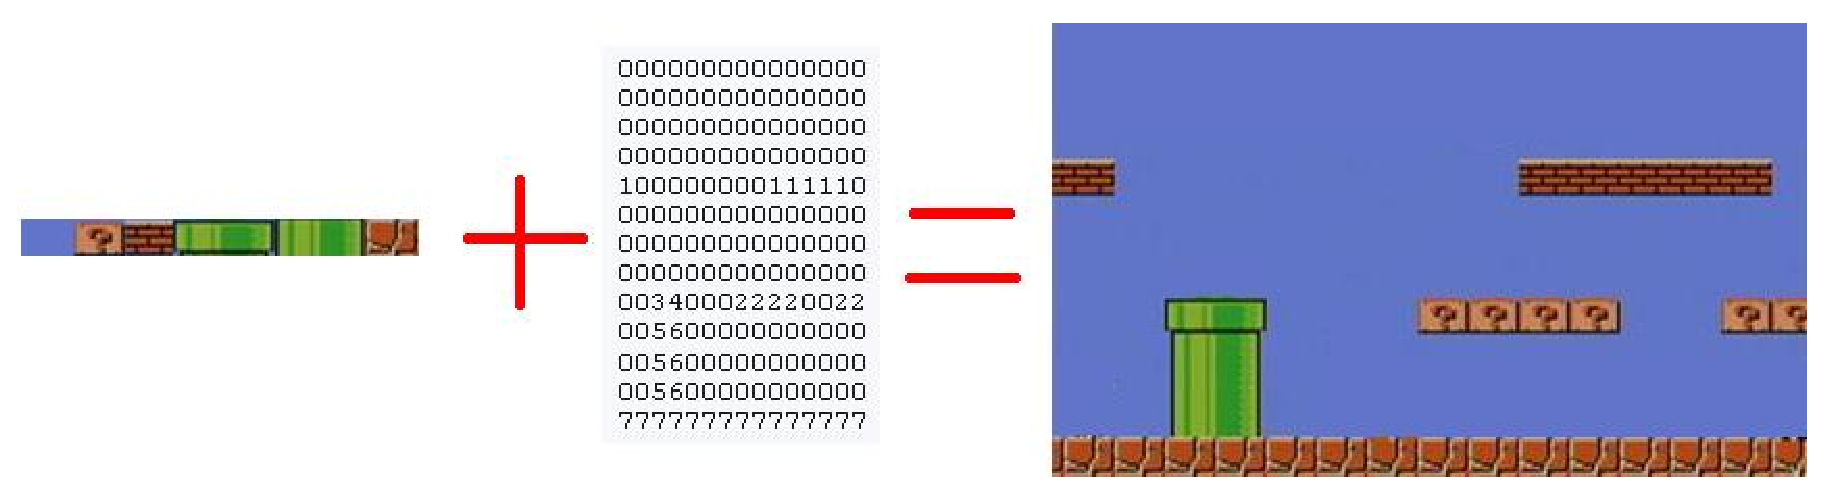
\includegraphics[width=15cm]{./Analyse/Img/tileMapping.eps}
		
		
		Nous avons donc repris ce principe et nous l'avons amélioré. En effet grâce à la programmation objet, les entiers sont réprésenté directement par des objets contenant le tile qui le représente. Ainsi, nous stockons dans une matrice tous les objets inanimés (les objets dont le tile restera le meme tout le long de la partie) et nous parcourons cette matrice pour dessiner chaque objet à sa position pour obtenir une nouvelle image au format png. Ainsi à chaque rafraichissement de l'écran, seule la nouvelle image est dessiné et non pas chaque tile. Cette méthode permet d'éviter un parcours intempestif de la matrice.
		Ensuite pour le reste des objets (les objets animés composés d'une sequence de tiles) nous avons décidé de les stocker dans une table de hachage dont la clé est la position de l'objet (pour y accéder plus rapidement). Ainsi à chaque rafraichissement de l'écran on va dessiner l'image des objets inanimés puis parcourir entierement la table de hachage et dessiner le tile courant de la sequence d'animation de chaque objet.
		
		\subsubsection{La gestion des images et du son}
		
		Chaque image, tile et chaque son dont est composé le jeu sont chargé au lancement de l'application. Tous les tiles sont stocké dans des images appelés sprites. Un sprite est donc un ensemble d'image. L'ensemble des tiles sont stockés dans différents sprites. Il y a un sprite pour les bombes, un pour les joueurs et un autre pour le reste des objets. Chaque sprite contient l'ensemble des images des objets qu'il représente. Chaque sprite est associé à un fichier \gls{xml}. Le fichier XML peut être réprésenté sous forme d'un arbre. Les fichiers XML ressemble tous plus au moins a ce genre d'arborescence: 
		
		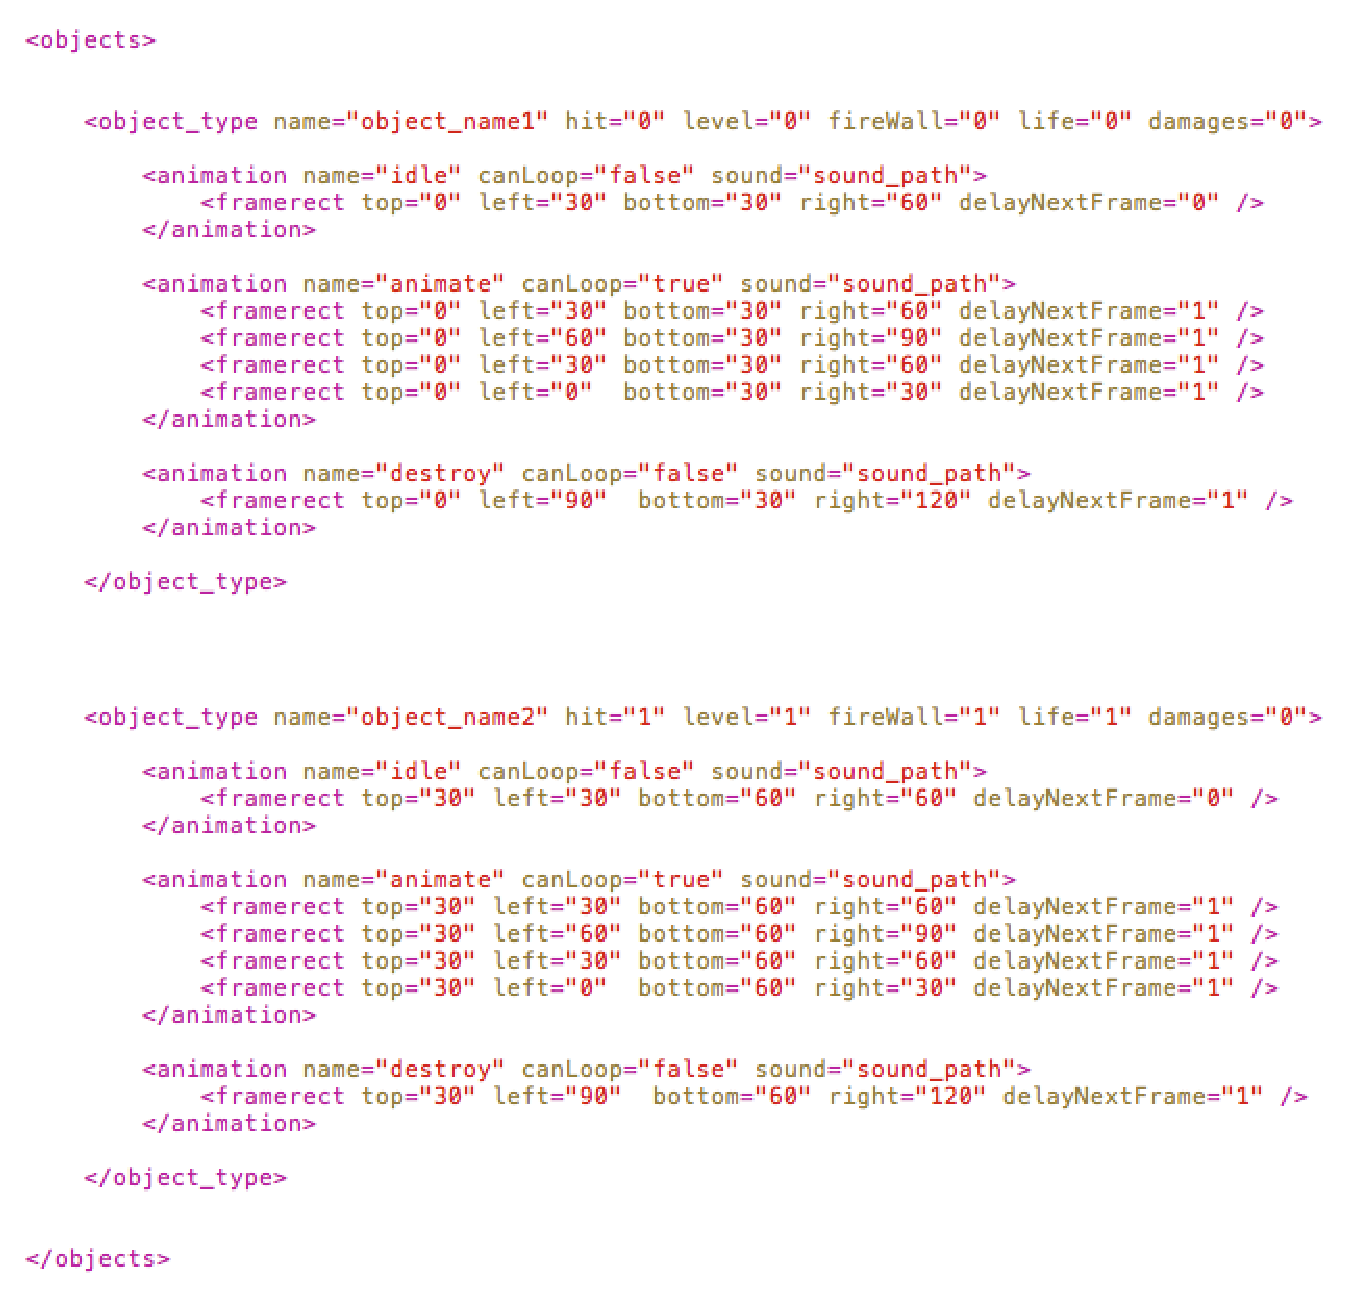
\includegraphics[width=15cm]{./Analyse/Img/exampleXmlBomberklob.eps}
		
		Chaque fichier XML commence par une balise racine permettant de lister les objets qu'elle contient (\textit{<objects>}). Ensuite chaque objet est décris par une balise  qui contient le type, le nom de l'objet ainsi que l'ensemble de ses propriétés. La propriété \textit{hit} est à 1 si l'objet peut être touché par une explosion (0, sinon), le champ \textit{level} est à 1 si l'objet est animés (0,sinon), le champ \textit{fireWall} est à 1 si l'objet ne laisse pas passer les flammes des explosions, le champ \textit{life} indique le nombre de fois que l'objet doit etre touché par des flammes pour qu'il soit entierement détruit, et enfin le champ \textit{damages} indique si l'objet peut infliger des domages. Par exemple \textit{<destructible name="herb" hit="1" level="1" fireWall="1" life="1" damages="0">} décris un objet de type \textit{destructible}, qui peut-etre touché par des flammes, qui est animé, ne laisse pas passer les flammes des bombes, possede une vie,  n'inflige pas de domage et dont le nom est \textit{herb} . Ensuite chaque objet possède au plus trois balises animations (sauf pour les joueurs). Tout objet possède au moins la premiere balise:  <animation name="idle" canLoop="false" sound="sound\_path"> qui est celle dont le nom est \textit{idle}. Elle représente l'image standard de l'objet. Par exemple pour un objet bombe, ce sera l'image qui sera affiché dans la liste des bombes pour pouvoir selectionner ses bombes. Le champs \textit{canLoop} permet de savoir si l'image doit être répété en boucle et le champ \textit{sound} contient le chemin d'acces au fichier de son de l'animation si elle en possede un. Il y a ensuite la même balise mais dont le nom est \textit{animate}, celle-ci contiendra toutes les sequences d'images d'un objet qui est animés. Puis la dernière est celle dont le nom est \textit{destroy}. Cette derniere contiendra l'ensemble des images composant la sequences d'animation de destruction de l'objet. Enfin chaque balise de type animation contient des balises de type \textit{framerect}. Ces balises permettent de donner la position de chaque image de la séquence d'animation dans le sprite ainsi que le delay de rafraichissement entre chaque image. Par exemple \textit{<framerect top="60" left="30" bottom="90" right="60" delayNextFrame="1" />} représente une image dont le bord du haut est situé à 30pixels, le bord du bas à 90pixels, le bord de gauche à 30pixels et le bord de droite à 60pixels en partant du coin en haut à gauche du sprite. Puis pour le champ \textit{delayNextFrame} celui-ci informe que l'image suivante sera déclenché apres un delay de 1s.\\
		
		Grâce à cette modélisation, l'application va parcourir au démarrage l'ensemble des fichiers XML et va créer une table de hachage pour chaque ensemble d'objet du fichier. Lors de ce parcours, l'application va instancier chaque objet avec toutes propriétés que lui indique le document XML, ainsi que ses sequences d'animation. Ensuite lorsqu'un objet devra être utilisé dans le jeu, il suffira d'utiliser une copie de l'objet déja chargé en mémoire pour éviter de devoir reparcourir le fichier.


\subsection{Réseau}
		
	\paragraph{Serveur\\}
			
		Il a été fixé dans le cahier des charges que notre serveur devrait pouvoir
		effectuer plusieurs tâches particulières séparées. Nous avons donc décidé de
		les compartimenter en classes.
		
		Notre serveur est crée sur une base de servlet. Ce fût ici
		aussi un point nouveau pour nous, réiterant les phases d'analyse, de
		découverte, de test et de mise en place. Le fonctionnement est basé sur les
		échanges de requêtes type HTTP, où à chaque demande correspond une réponse. 
		
		Une servlet est une classe Java qui permet de créer dynamiquement des données
		au sein d'un serveur HTTP. Une servlet s'exécute dynamiquement sur le serveur
		web et permet l'extension des fonctions de ce dernier, typiquement : accès à
		des bases de données.
			
		Les six éléments situés sur la partie haute du schéma
		ci-dessous(respectivement ServletInscription, ServletConnection,
		ServletGamesList, ServletCreateGame, ServletConnectionGame et
		ServletManageGame), représente les différentes tâches qu'un utilisateur
		puisse demander au serveur. Elles sont reliées à une classe nommée
		ContextListener, qui leur permettra d'accéder aux mêmes données sans qu'il y
		ait de conflits. La partie basse représente les objets qui seront utilisés pour les parties en multijoueurs. 
		Bien évidemment ces objets sont très proches de ceux utilisés dans les parties
		locales(Schéma 3.3).
		
		
		Comme il a été dit précédement, notre serveur est accessible via des requêtes
		HTTP contactant des servlets. Ces servlets sont stockées dans un serveur
		d'application nommé Apache Tomcat. Il s'agit d'un conteneur libre de
		servlets Java 2 Enterprise Edition, mais il fait aussi office de serveur
		Web.\\
		
		
		Le scénarios le plus probable serait le suivant. Un utilisateur désire jouer
		en ligne contre de vrais joueurs. 
		Il va alors passer par l'inscription et créer son compte sur le
		serveur(Inscription). Une fois cette étape obligatoire faite, il pourra
		choisir entre rejoindre une partie en ligne en cour(ConnectionGame), ou en
		créer un nouvelle(CreateGame). Dès lors qu'il aura accès à une partie en
		ligne, un contact régulier avec le serveur sera obligatoire afin de réaliser
		les interactions entre les différents joueurs(ManageGame). Tout ceci devra se
		réaliser bien sûr dans une durée infime afin de ne pas pénaliser les joueurs.	
		
		\begin{figure}
			\includegraphics[scale = 0.5]{Analyse/Img/serveur.eps}
			 \caption {Serveur}
		\end{figure}
		
		\newpage
		
		
	\paragraph{JSON\\}	
		Soucieux des performances et de la rapidité des échanges entre applications et
		serveur, nous avons mis en place un protocole de communication client/serveur
		où les messages transitant sont des flux \gls{json}. 	
		Contrairement au \gls{xml} qui peut représenter des données orientées document,
		\gls{json} se focalise sur la description d’objets.
		Un autre avantage reconnu de \gls{json} par rapport à \gls{xml} est qu’il est nettement
		moins verbeux que ce dernier.
		Quoi qu’il en soit \gls{json} reconnait la philosophie des services web exposant
		une interface d’échange : il s’agit
		d’envoyer et de recevoir des informations dans un format facilement manipulable par
		le protocole de transport \gls{http}.
		
		
		Voilà pourquoi le \gls{json} semblait être un format de données d'échanges optimal
		pour véhiculer le plus d'informations avec une taille moindre. Il est aussi en
		adéquation avec notre politique d'utilisation web pour un serveur.
		De plus étant beaucoup utilisé, nos deux
		langages mettent à disposition des outils de sérialisation de leurs objets en \gls{json}
		
		Ci-dessous un exemple concret de notre protocole de communication \gls{json} entre
		serveur et application cliente.
		
			
		\begin{verbatim}
			ServletInscription
				Player => Serveur
				{["username","password"]}
				
				Serveur => Player
				{"OK"} ou {"BU"}
				
			ServletConnexion 	
				Player => Serveur
				{["username","password"]}
				
				Serveur => Player
				{"OK"} ou {"BU"}
				
			ServletGameList
				Player => Serveur
				{"userKey"}
			
				Serveur => Player
				{[{"class":"Game","map":"mapName","name":"gameName",
				 "playerNumberConnected":nbConnected,"type":"gameType"},{..},{..}]}
				 
			ServletCreateGame:
				Player => Server:
					{"userKey": <userKey>, 
					"game": {"name":<name>, "type":<type>, "map":<map>, "ennemiesNumber": <ennemiesNumber>}}
					
				Server => Player:
					{"OK"} ou {"errorType"}
				 
			ServletConnectionGame:
				Player => Server:
					{["userKey", "gameName"]}
					
				Server => Player:
					{[<1/2/3/4>, "play<true/false>", "map", "time<mm:ss>"]} 
					ou 
					{"errorType"}
					
			ServletManageGame:
				Player => Server: 
					{"userKey", "gameName", "action"}	
					
				Server => Players: (Player, bombs, blocs, score, time)
					{[
					 [ ["x", "y", "direction", "dead <true/false>"],[...] ],
					 [ ["x", "y", "type", "explode <true/false>" ], [...] ],
					 [ ["position": {"x", "y"}, "bonus": <bonus>], [..] ],
					 [1,2,3,4],
					 "time <mm:ss>"]} 
					 ou 
					{"errorType"}
				 
				 
		\end{verbatim}
			
		
	

	\subsubsection{Schéma de fonctionnement }
		
		\begin{center}
			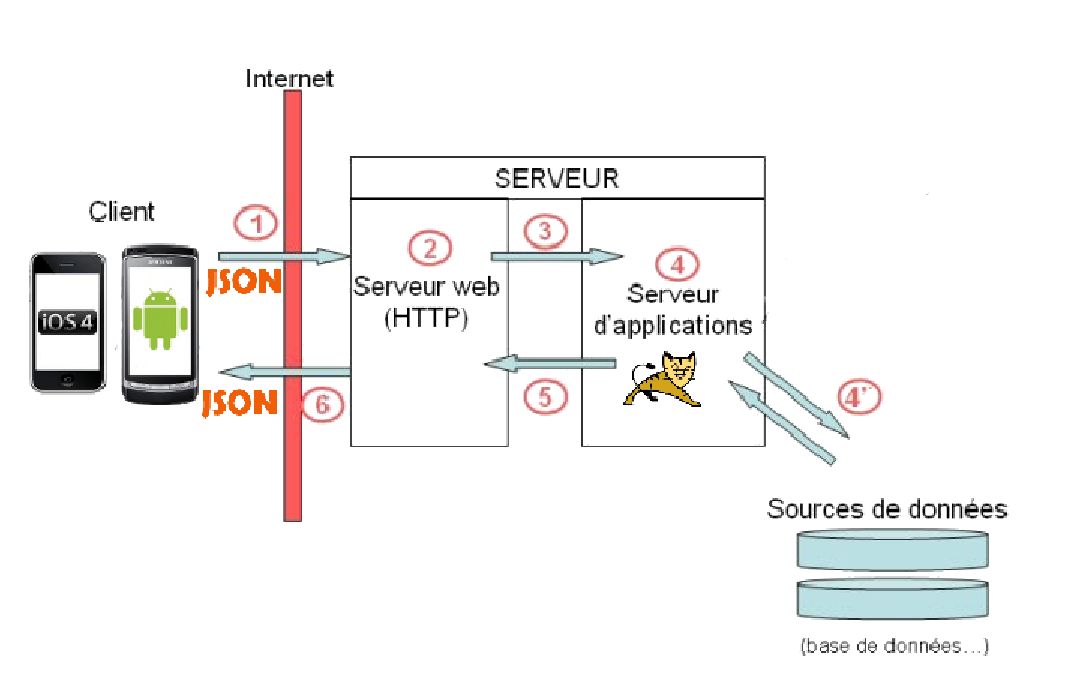
\includegraphics[width=16cm]{Analyse/Img/serveurappli.eps}
		\end{center}
		
		\begin{enumerate}

			\item 
					Le client émet une requête pour demander une
					ressource au serveur. Par exemple la création de son compte multijoueur,
					qui pourrait se situer \url{http://Bomberklob.com/inscription}
			\item
					Côté serveur, c'est le serveur web qui traite les
					requêtes HTTP entrantes. Il traite donc toutes les requêtes, qu'elles
					demandent une ressource statique ou dynamique. Seulement, un serveur HTTP
					ne sait répondre qu'aux requêtes visant des ressources statiques.

			\item 
					Ainsi, si le serveur HTTP s'aperçoit que la requête reçue est destinée
					au serveur d'applications, il la lui transmet. Les deux serveurs sont
					reliés par un canal, nommé connecteur.
		
			\item
					Le serveur d'applications (dans notre cas Tomcat) reçoit la requête à
					son tour. Lui est en mesure de la traiter. Il exécute donc la servlet
					correspondante à la requête, en fonction de l'URL, en récupérant les
					valeurs dans le flux JSON entrant. Cette opération est effectuée à partir
					de la configuration du serveur, grâce un fichier web.xml faisant le mapping
					entre URL et servlet associée.
		
					La servlet est donc invoquée, et le serveur lui fournit notamment deux
					objets Java exploitables: un représentant la requête, l'autre représentant
					la réponse. La servlet execute sa fonction et génère la réponse à la
					demande, sous forme de flux JSON. Cela peut passer par la consultation de
					sources de données, comme des bases de données (4' sur le schéma).		
		
		\end{enumerate}
		
	\paragraph{Base de données\\}
		Afin de pouvoir conserver les utilisateurs en ligne ainsi que leurs infos
		personnels et permettre une authentification, nous avons dû établir une
		base de données sur le serveur. Cette dernière à été pensé comme demandé pour 
		l'enregistrement de comptes. Une unique table nommée Users remplie donc cette
		fonction. Le serveur devra pouvoir y accéder en écriture(inscription) comme
		en lecture(connexion).
			Aléatoire
		Elle ne comportera que deux champs, userName et password. Dès lors que
		l'utilisateur désirera créer un compte multijoueur, il renseignera dans
		l'application son userName souhaité ainsi que son mot de passe. 
		Ce couple sera 	alors envoyé au serveur qui vérifiera dans cette base de
		données, que le userName(unique) n'est pas déjà utilisé. Auquel cas un nouveau n-uplet sera
		inséré et permettra l'authentification de l'utilisateur par la suite. Les mots
		de passe seront bien évidement crypté pour des raisons de sécurité.
			

		\newpage
		
	
						
\section{Différences entre Android et iOS}
	Lors du développement sous en \gls{android} et \gls{ios}, nous avons été
 confronté à divers problèmes.
Notamment des problèmes liés aux différences entre ces deux \glspl{os}.
Dans un premier temps, le langage utilisé n'est pas le même, le premier utilise
 le langage \gls{java} alors que l'autre utilise l'\gls{objective-c}.
 Ces deux langages étant des langages orientés objets, la difficulté réside
 surtout dans la différence de la syntaxe.
Ensuite, lors de l'implémentation de notre diagramme de classe notre premier
 soucis a été les différences de modélisation des vues et des controlleurs.
 En effet sous \gls{android}, les écouteurs d'une vue sont directement situés
 dans le controlleur de cette dernière alors que sous \gls{ios} les écouteurs
 peuvent être implémentés soit dans la vue soit dans son controlleur.
Pour respecter au maximum le modèle \gls{mvc}, nous avons choisi de placer les
écouteurs dans la vue sous \gls{ios} (ce qui est recommandé par Apple). 
	


\chapter{Développement}

	\section{Mobile}
	\subsection{Menus}
	\subsubsection{API et widget}

			TODO ludo
		
	\subsubsection{BDD}

		Après avoir effectué divers recherches, il s'est avéré que les mobiles
		utilisent un moteur de base de données relationnelles, accessible par le
		langage SQL. Dans notre cas il s'agit de SQLite 3. Sa particularité est de ne
		pas reproduire le schéma habituel client-serveur mais d'être directement intégrée au programme.
		L'accès à la base de données SQLite se fait par l'ouverture du fichier
		correspondant à celle-ci : chaque base de données est enregistrée dans un fichier qui lui est propre,
		 avec ses déclarations, ses tables, ses index mais aussi ses données.
			
		\paragraph{Android\\}
			
			Pour manipuler aisément les bases de données depuis l'application,
			nous avons crée une classe héritant de \textit{SQLiteOpenHelper}. Cette
			dernière fournit des outils de manipulations. Un attribut y est
			instancié, il s'agit de la base de données elle même, de type
			\textit{SQLiteDatabase}.
			
			Nous y avons crée 3 tables, \textit{PlayerAccount} sauvegardant toutes les
			informations sur les utilisateurs locaux, \textit{System} concervant les
			propriétés du système, et enfin \textit{Map} décrivant les informations
			relatives au cartes de jeu crées par l'utilisateur.
			
			Ainsi de nombreuses	fonctions ont été implémenté dans le but de simplifier les interactions
			avec cette base de données depuis l'application. Il est par exemple possible de créer un nouvel 
			utilisateur local, modifier ses préférences, gérer les configurations systèmes comme la langue ou le volume
			du son, ajoûter de nouvelles maps ou même récupérer toutes les informations
			concernant un utilisateur.\\
			
			Voici un exemple d'insertion d'un nouveau compte local dans la base de
			donnée. Rappelons que les tests d'existance du compte ont été fait depuis
			l'application même. Dans cet exemple vous verrez ainsi que nous commençons
			par récupérer les droits en écritures sur la base de données locale, puis
			nous créons un container qui servira à l'insertion de valeur dans la base. Et
			enfin l'insertion est faite. Nous terminons tout de même en fermant l'accès à
			cette base.
			
			Il s'agit la d'un schéma classique de fonction d'interaction avec notre
			base.
						
			\begin{verbatim}
			/** ajout compte hors ligne **/
				public long newAccount(String nomCompte){
					base = getWritableDatabase();
			
					ContentValues entree = new ContentValues();
					
					entree.put("pseudo", nomCompte);
					long var = base.insert("PlayerAccount", null, entree);
					
					base.close();
					return var;
				}
			\end{verbatim}

			
		\paragraph{iOS}
				
	\subsubsection{Première utilisation}
	\subsubsection{Création utilisateur}
	\subsubsection{Gestion utilisateur}
	\subsubsection{Gestion des préférences système}
	\subsubsection{Création de carte (charger)}
	\subsubsection{Création partie solo (tout)}
	\subsubsection{Création partie multi (officielle)}
			

\subsection{Editeur de carte}
	\subsubsection{Rendu}
		\subsubsection{Interface utilisateur}
		\subsubsection{Sauvegarde}


\subsection{Jeu}
	\subsubsection{Moteurs}
		\paragraph{Rendu}
			\subparagraph{Structure utilisée}
				\begin{itemize}
					\item{Pourquoi}
					\item{Avantages}
				\end{itemize}
		\paragraph{Physique}
			\subparagraph{Structure utilisée}
			\subparagraph{Mouvements (collisions)}
			\subparagraph{Gestion des bombes}
				\begin{itemize}
					\item{Threads}
				\end{itemize}
	
	\subsubsection{IA}
		\paragraph{Pathfinding}
			\subparagraph{A*}
			\subparagraph{Aléatoire}
			\paragraph{Prise de décision}
	
	\subsubsection{Interface utilisaeur}
		\paragraph{Android}
		\paragraph{iOS}
		
		
\section{Serveur}
	Nous avons choisi de créer notre serveur sur une base de servlet. Ce fût ici
aussi un point nouveau pour nous, réiterant les phases d'analyse, de
découverte, de test et de mise en place. Le fonctionnement est basé sur les
échanges de requêtes type HTTP, où à chaque demande correspond une réponse. 
		
\subsection{Json}
	Soucieux des performances et de la rapidité des échanges entre applications et
	serveur, nous avons mis en place un protocole de communication client/serveur
	où les messages transitant sont des flux JSON. Ce dernier semblait être un
	format de données d'échanges optimal pour véhiculer le plus d'informations
	avec une taille moindre. De plus étant beaucoup utilisé, nos deux langages
	mettent à disposition des outils de sérialisation de leurs objets en JSON.
		
	\begin{verbatim}
		ServletInscription
			Player => Serveur
			{["username","password"]}
			
			Serveur => Player
			{"OK"} ou {"BU"}
			
		ServletConnexion 	
			Player => Serveur
			{["username","password"]}
			
			Serveur => Player
			{"OK"} ou {"BU"}
			
		ServletGameList
			Player => Serveur
			{"userKey"}
		
			Serveur => Player
			{[{"class":"Game","map":"mapName","name":"gameName",
			 "playerNumberConnected":nbConnected,"type":"gameType"},{..},{..}]}
			 
		ServletCreateGame:
			Player => Server:
				{"userKey": <userKey>, "game": {"name":<name>, "type":<type>, "map":<map>, "ennemiesNumber": <ennemiesNumber>}}
				
			Server => Player:
				{"OK"} ou {"errorType"}
			 
		ServletConnectionGame:
			Player => Server:
				{["userKey", "gameName"]}
				
			Server => Player:
				{[<1/2/3/4>, "play<true/false>", "map", "time<mm:ss>"]} 
				ou 
				{"errorType"}
				
		ServletManageGame:
			Player => Server: 
				{"userKey", "gameName", "action"}	
				
			Server => Players: (Player, bombs, blocs, score, time)
				{[
				 [ ["x", "y", "direction", "dead <true/false>"],[...] ],
				 [ ["x", "y", "type", "explode <true/false>" ], [...] ],
				 [ ["position": {"x", "y"}, "bonus": <bonus>], [..] ],
				 [1,2,3,4],
				 "time <mm:ss>"]} 
				 ou 
				{"errorType"}
			 
			 
	\end{verbatim}
		
\subsection{Servlet}
	Comme il a été dit précédement, notre serveur est accessible via des requêtes
	HTTP contactant des servlets. Ces servlets sont stockées dans un serveur
	d'application nommé Apache Tomcat. Il s'agit d'un conteneur libre de
	servlets Java 2 Enterprise Edition, mais il fait aussi office de serveur Web.
		
	Une servlet est une classe Java qui permet de créer dynamiquement des données
	au sein d'un serveur HTTP. Une servlet s'exécute dynamiquement sur le serveur
	web et permet l'extension des fonctions de ce dernier, typiquement : accès à
	des bases de données.
		

	\subsubsection{Schéma de fonctionnement }
		
		\begin{center}
			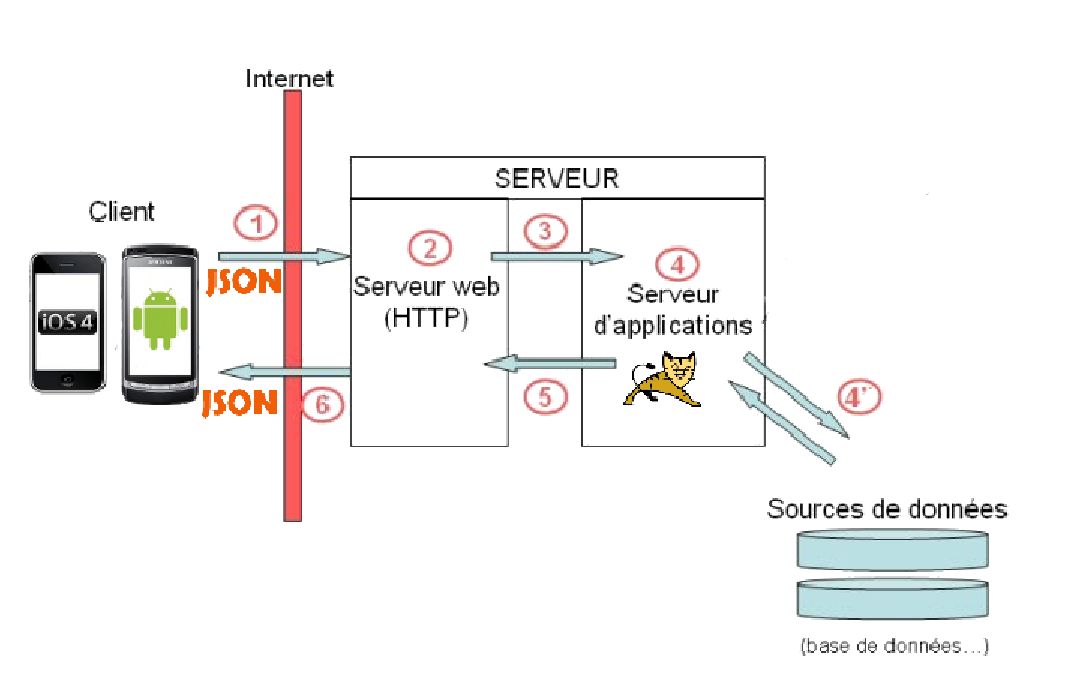
\includegraphics[width=16cm]{Analyse/Img/serveurappli.eps}
		\end{center}
		
		\begin{enumerate}

			\item 
					Le client émet une requête pour demander une
					ressource au serveur. Par exemple la création de son compte multijoueur,
					qui pourrait se situer \url{http://Bomberklob.com/inscription}
			\item
					Côté serveur, c'est le serveur web qui traite les
					requêtes HTTP entrantes. Il traite donc toutes les requêtes, qu'elles
					demandent une ressource statique ou dynamique. Seulement, un serveur HTTP
					ne sait répondre qu'aux requêtes visant des ressources statiques.

			\item 
					Ainsi, si le serveur HTTP s'aperçoit que la requête reçue est destinée
					au serveur d'applications, il la lui transmet. Les deux serveurs sont
					reliés par un canal, nommé connecteur.
		
			\item
					Le serveur d'applications (dans notre cas Tomcat) reçoit la requête à
					son tour. Lui est en mesure de la traiter. Il exécute donc la servlet
					correspondante à la requête, en fonction de l'URL, en récupérant les
					valeurs dans le flux JSON entrant. Cette opération est effectuée à partir
					de la configuration du serveur, grâce un fichier web.xml faisant le mapping
					entre URL et servlet associée.
		
					La servlet est donc invoquée, et le serveur lui fournit notamment deux
					objets Java exploitables: un représentant la requête, l'autre représentant
					la réponse. La servlet execute sa fonction et génère la réponse à la
					demande, sous forme de flux JSON. Cela peut passer par la consultation de
					sources de données, comme des bases de données (4' sur le schéma).		
		
		\end{enumerate}
		
		
	\subsubsection{En pratique}
		
		Le requetes font appel à la fonction post des servlet. Le flux entrant étant
		de type JSON, il faut déserialiser le flux dans un objet correspondant. Exemple
		l'utilisateur envoie son userName et son mot de passe crypté dans un tableau,
		sérialisé en JSON, pour pouvoir récupérer les informations nous procédons
		comme suit: 
		
		\begin{verbatim}
			BufferedReader req = 
				  new BufferedReader(new InputStreamReader(request.getInputStream()));
			OutputStreamWriter writer = 
				  new OutputStreamWriter(response.getOutputStream());
			String message = req.readLine();
			
			if (message != null) {
				  response.setContentType("text/html");
				
				   // désérialisation des infos de l'utilisateur dans une arraylist 
				  JSONDeserializer<ArrayList<String>> jsonDeserializer = 
					  new JSONDeserializer<ArrayList<String>>();
				  ArrayList<String> identifiers;
				  identifiers = jsonDeserializer.deserialize(message);
				
				  username = identifiers.get(0);
				  password = identifiers.get(1);
				  
			  ...}
		\end{verbatim}
		
		
	\subsubsection{La sécurité}
	
		Ce serveur de jeu étant hebergé sur internet et contenant des informations
		sensibles d'utilisateurs, tels que des mots de passes, il était crucial
		d'instaurer des règles de sécurité et de cryptage. 
		
		En effet lors des inscriptions ou connexion au serveur pour le mode
		multijoueur, les mots de passes sont tout d'abord cryptés côté client et
		ensuite encapsulé dans un flux JSON, pour être envoyé au serveur. Il stockera
		ainsi la chaine de caractères extraite de l'objet déserialisé. De cette
		manière à aucun moment les données confidentielles ne transiteront en clair.
		
		De plus un mécanisme de session est en place. Dans la confirmation de
		connexion ou d'inscription, une userKey est générée. Elle correspond en
		réalité à l'identifiant de session envoyé par le serveur. Une fois associée
		à l'username correspondant, le tout est ajoûté dans le tableau d'utilisateurs
		connectés.
		Cet userKey est ensuite nécessaire pour contacter les servlets suivantes. Si
		cet identifiant n'est pas envoyé ou n'est pas présent dans le tableaux des
		utilisateurs connectés, il sera alors impossible d'accéder aux ressources du
		serveur.
		
\subsection{BDD}

	La base de données du serveur n'est pas très complexe. En effet elle ne fait
	qu'accueillir les couples userName/password des utilisateurs dans la
	table Users. 
	Pour son accès, chaque servlet peut récupérer un objet de type Connection,
	instancié à l'initialisation du serveur. Il permettra à son tour
	de récuperer un objet de type Statement. L'application va l'employer pour
	transmettre des instructions à la base. Exemple d'insertion: 
		
	\begin{verbatim}
		Statement theStatement = connection.createStatement();
		theStatement.execute(
		     "INSERT into Users VALUES ('"+ username +"','"+password+"')");
	\end{verbatim}


	
		
		
		
		
\chapter{Manuel d'utilisation}

	\section{Menus}
	

\subsection{Premier lancement}

	%\paragraph{Chargement\\}
	%Une première image de chargement apparaît au lancement de l'application. Cette
	%animation reste un certain temps suivant la rapidité du mobile.
	
	%\begin{figure}[h]
	%	\centering
	%		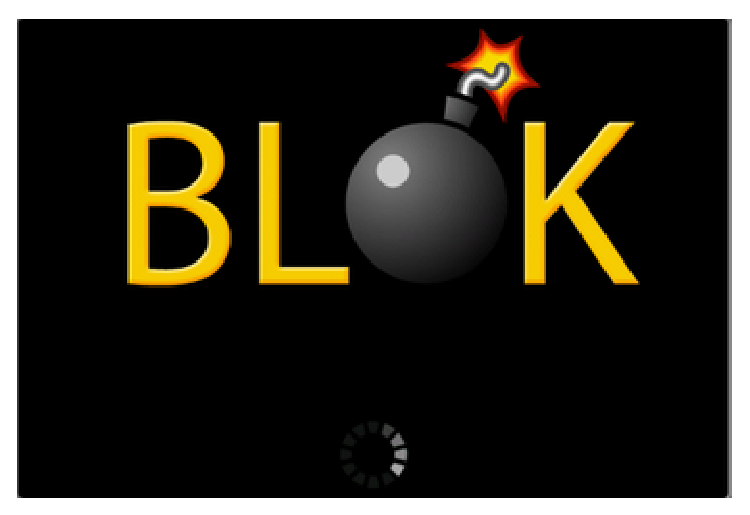
\includegraphics[scale=0.7]{Manuel/Img/1}
		%	\caption{Chargement}
	%	\end{figure}			
		
	\paragraph{Création compte local\\}
	Au premier lancement de l'application il vous est demandé de créer un compte un
	local. Ce dernier est nécessaire pour pouvoir utiliser l'application. Il vous
	suffira de renseigner dans le champs prévu à cet effet, votre pseudonyme 1).
	\begin{figure}[h]
	\centering
			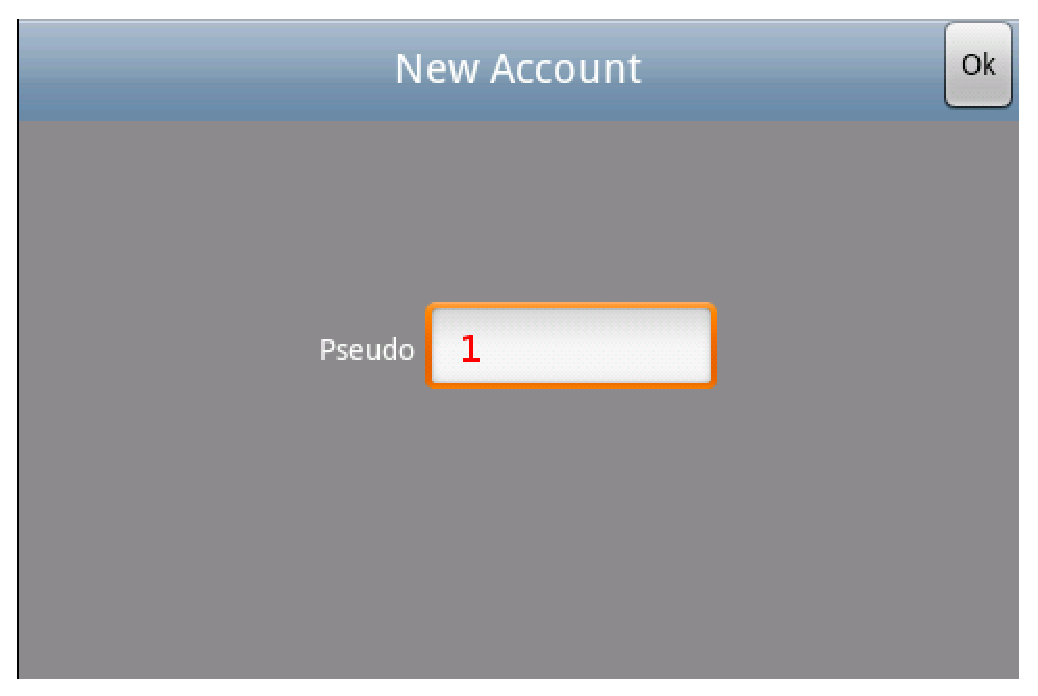
\includegraphics[scale=0.6]{Manuel/Img/2.eps}
			\caption{Création compte local}
	\end{figure}

	
\subsection{Menu}	
	Le menu d'accueil vous permet d'accéder à la section des parties locales
	\textcolor{red}{\textbf{1}}, des parties multijoueurs
	\textcolor{red}{\textbf{2}}, l'éditeur de carte \textcolor{red}{\textbf{3}}
	pour créer vos propres cartes de jeu, le menu d'options
	\textcolor{red}{\textbf{4}}, l'accès aux comptes locaux
	\textcolor{red}{\textbf{5}}, la création d'un nouveau compte local
	\textcolor{red}{\textbf{6}} et enfin l'aide \textcolor{red}{\textbf{7}}.
	\begin{figure}[h]
		\centering
			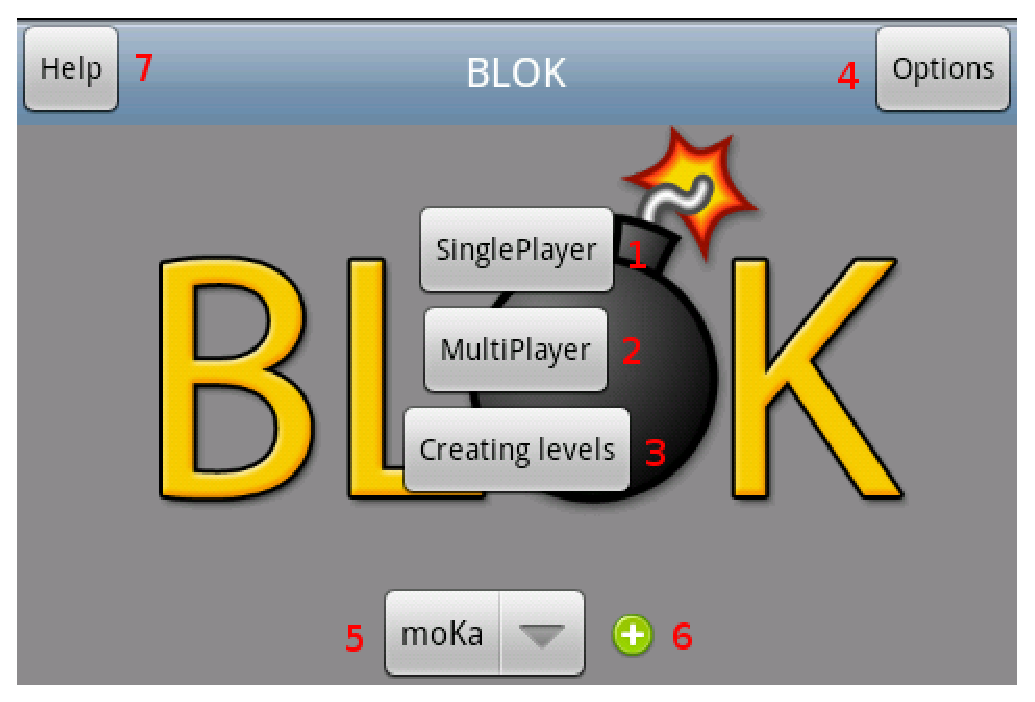
\includegraphics[scale=0.7]{Manuel/Img/3.eps}
			\caption{Ajoût nouveau compte local}
	\end{figure}
	
	
	
	\subsection{Jeu local \textcolor{red}{1}}
	\paragraph{Paramétrage\\}
	Voilà un moment crucial précédent votre lancement de jeu, sa configuration.
	Rien de bien compliqué en soit, vous choisissez le type de partie
	\textcolor{blue}{\textbf{1}}, la difficulté de vos adversaires(robots)
	\textcolor{blue}{\textbf{2}}, le nombre d'ennemis sur la carte
	\textcolor{blue}{\textbf{3}}, et le temps de jeu \textcolor{blue}{\textbf{4}},
	et enfin grâce à un défilement de la galerie \textcolor{blue}{\textbf{5}}, la
	carte de jeu, et enfin vous validez \textcolor{blue}{\textbf{6}}.
	
	\begin{figure}[h]
	\centering
		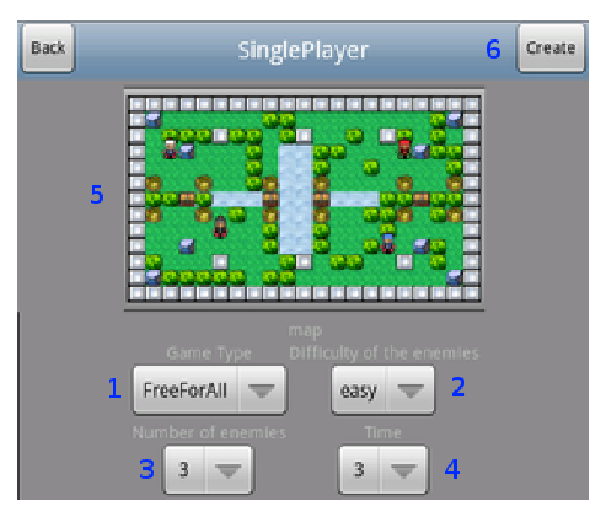
\includegraphics[scale=0.7]{Manuel/Img/15.eps}
		\caption{Paramétrage partie locale}
	\end{figure}
	
	\paragraph{Jeu\\}
	Après avoir choisi vos préférences pour votre partie, celle-ci se lance.
	Pour vous déplacer votre joueur effleurez l'écran de jeu dans le sens et la
	direction vous souhaiter aller \textcolor{blue}{\textbf{1}} .	
	Sur le panneau de droite en appuyant sur le
	bouton prévu \textcolor{blue}{\textbf{2}}, vous posez des bombes.
	Le panneau du haut résume les informations de la partie. Le temps de jeu
	\textcolor{blue}{\textbf{3}} restant, et vos différents bonus . Ces derniers
	correspondants à la portée de vos bombes \textcolor{blue}{\textbf{4}}, le
	nombres de bombes que vous pouvez poser
	simultanément \textcolor{blue}{\textbf{5}} , la vitesse de déplacement de votre
	joueur \textcolor{blue}{\textbf{6}}, et votre compteur de vies
	\textcolor{blue}{\textbf{7}}.
	
	\begin{figure}[h]
	\centering
		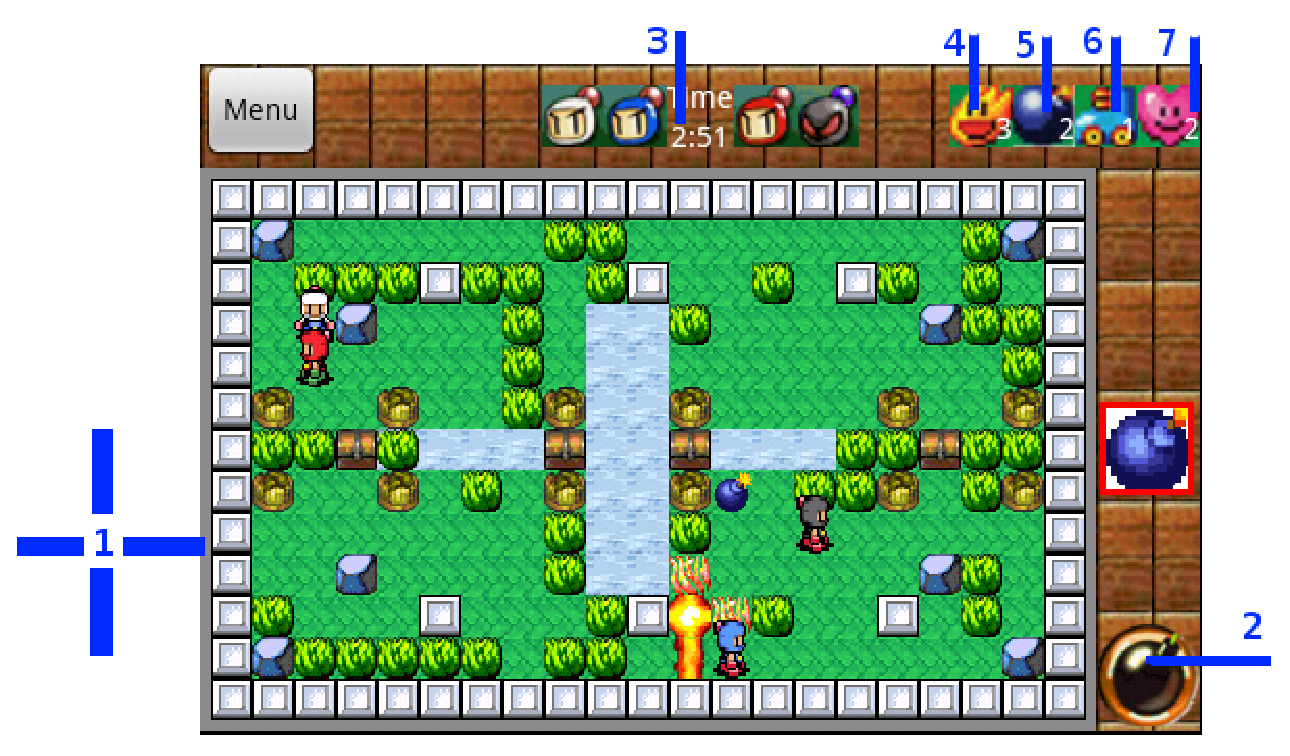
\includegraphics[scale=0.6]{Manuel/Img/21.eps}
		\caption{Jeu en cour}
	\end{figure}
	
	\paragraph{Pause\\}
	Lors d'une partie vous pouvez la suspendre en appuyant sur le Menu
	\textcolor{orange}{\textbf{1}} en haut à gauche. Il vous est possible de
	reprendre la partie \textcolor{orange}{\textbf{2}}, accéder aux options de jeu
	\textcolor{orange}{\textbf{3}}, redémarrer la partie
	\textcolor{orange}{\textbf{4}}, ou tout simplement la quitter et revenir au
	menu \textcolor{orange}{\textbf{5}}. 
	
	\begin{figure}[h]
	\centering
		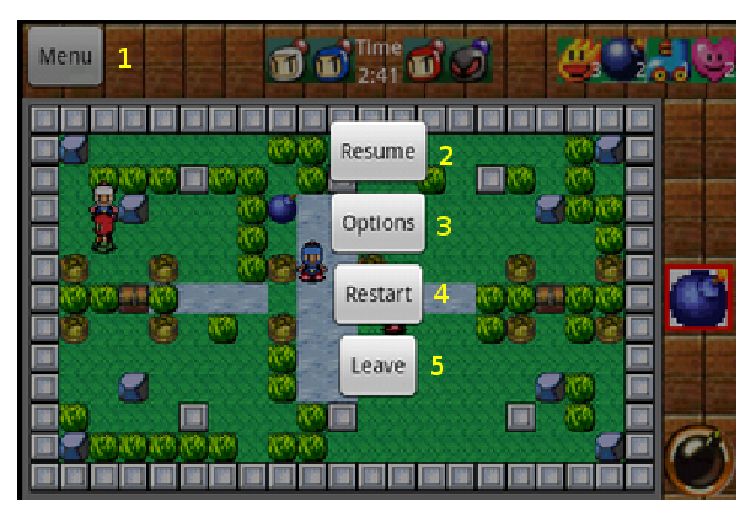
\includegraphics[scale=0.7]{Manuel/Img/20.eps}
		\caption{Pause lors d'une partie}
	\end{figure}


\subsection{Jeu multi \textcolor{red}{2}}

	\paragraph{Inscription}
	Cette étape est inévitable afin d'accéder au mode multijoueur. Vous devez
	renseigner userName \textcolor{blue}{\textbf{1}}, mot de passe
	\textcolor{blue}{\textbf{2}}, et confirme ce dernier
	\textcolor{blue}{\textbf{3}}. Vous pouvez choisir une connexion automatique
	\textcolor{blue}{\textbf{4}} ou simplement ne pas ressaisir votre mot de passe
	aux connexions suivantes \textcolor{blue}{\textbf{5}}. Dès que ces champs sont
	remplis, validez via la connexion au serveur \textcolor{blue}{\textbf{6}}. Le
	userName est unique, s'il est déjà pris le serveur vous renverra une erreur,
	sinon vous accéderez à l'Accueil du mode multijoueur.
	
	
	\begin{figure}[h]
	\centering
		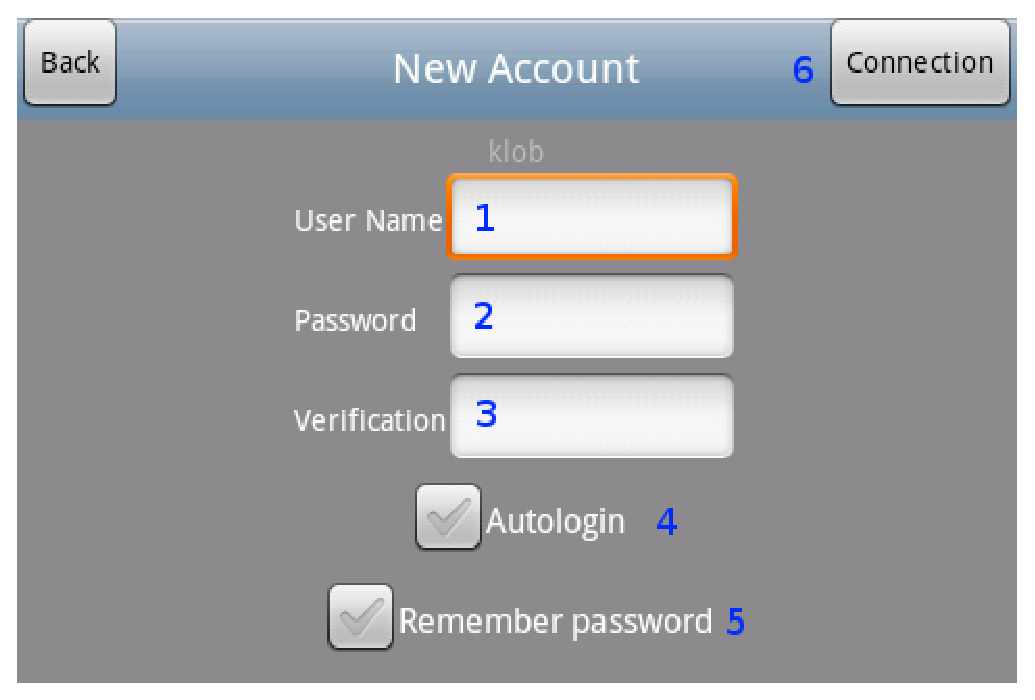
\includegraphics[scale=0.7]{Manuel/Img/18.eps}
		\caption{Création compte multijoueur}
	\end{figure}
	
	\paragraph{Connexion}
		Une fois seulement l'étape précédente accomplie vous devrez passer par le menu
		de connexion. Dans ce dernier il faut donner le couple
		userName \textcolor{blue}{\textbf{1}}/mot de passe
		\textcolor{blue}{\textbf{2}}, et vous pouvez aussi choisir, dans le cas d'une
		identification correcte, la mémorisation de votre complet
		\textcolor{blue}{\textbf{3}} c'est à dire un accès direct sans passer par le
		menu de connexion, ou la mémorisation unique de votre mot de passe
		\textcolor{blue}{\textbf{4}}. Enfin il est toujours possible de créer un
		nouveau compte multijoueur \textcolor{blue}{\textbf{5}}. Là encore une
		vérification sur le serveur est faite lorsque vous choisirez la connexion
		\textcolor{blue}{\textbf{6}}.
		
	\begin{figure}[h]
	\centering
		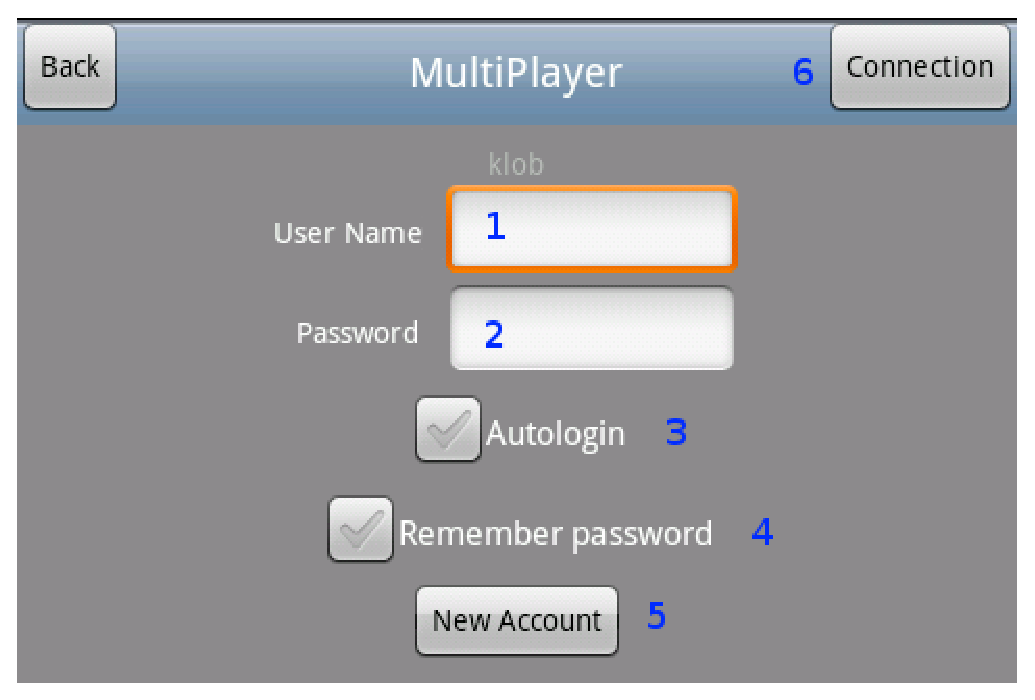
\includegraphics[scale=0.7]{Manuel/Img/17.eps}
		\caption{Connexion compte multijoueur}
	\end{figure}
	
	\paragraph{Accueil}
	L'accueil du mode multijoueur est composé d'un champ éditable, permettant le
	tri des parties en lignes \textcolor{blue}{\textbf{1}}, le rafraichissement des
	parties \textcolor{blue}{\textbf{2}}, une liste déroulante clickable de celles
	en cour \textcolor{blue}{\textbf{3}}, et enfin un accès au menu de création
	d'une nouvelle \textcolor{blue}{\textbf{4}}.
	
	\begin{figure}[h]
	\centering
		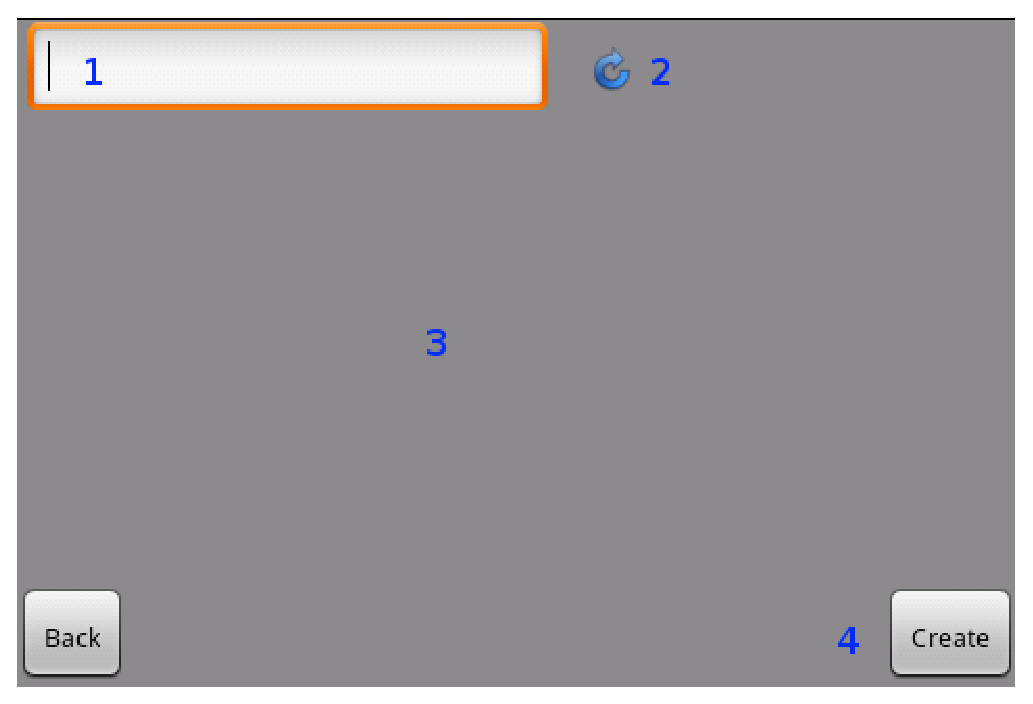
\includegraphics[scale=0.7]{Manuel/Img/19.eps}
		\caption{Accueil des parties multijoueurs}
	\end{figure}
	
	\paragraph{Créer partie}
	La création multijoueur et semblable à celle en locale.
	Vous choisissez le type de partie
	\textcolor{blue}{\textbf{1}}, la difficulté de vos adversaires(robots)
	\textcolor{blue}{\textbf{2}} en attendant les vrais joueurs , le nombre d'ennemis
	sur la carte \textcolor{blue}{\textbf{3}}, et le temps de jeu \textcolor{blue}{\textbf{4}},
	et enfin grâce à un défilement de la galerie \textcolor{blue}{\textbf{5}}, la
	carte de jeu, et finalement vous validez \textcolor{blue}{\textbf{6}}.
	
	\begin{figure}[h]
	\centering
		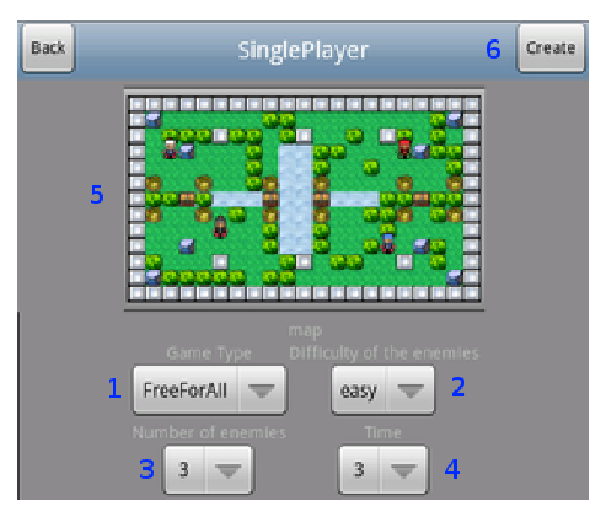
\includegraphics[scale=0.7]{Manuel/Img/15.eps}
		\caption{Création partie multijoueur}
	\end{figure}
	
	
\subsection{Editeur de map \textcolor{red}{3} }
	
	\paragraph{Création de map\\}
	Comme dans tout jeux d'arcade qui se respecte, vous avez la possibilité de
	créer vos niveaux via un éditeur. Vous n'avez qu'à donner le nom de la carte
	\textcolor{blue}{\textbf{1}}	que vous souhaitez créer puis valider
	\textcolor{blue}{\textbf{2}}. La encore les doublons ne sont pas possibles.
	
	\begin{figure}[h]
		\centering
			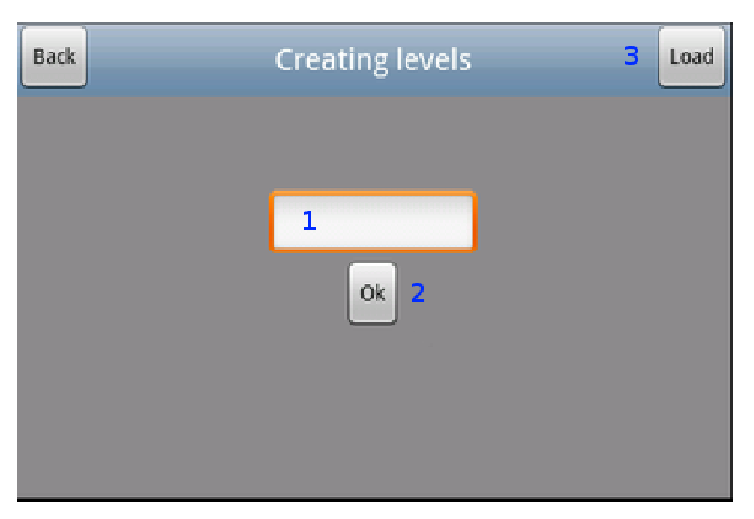
\includegraphics[scale=0.7]{Manuel/Img/10.eps}
			\caption{Création de map}
		\end{figure}

	
	\paragraph{Edition de map\\}
	Une carte vierge s'offre à vous \textcolor{blue}{\textbf{1}}. Le choix des
	structures(destructibles ou non) \textcolor{blue}{\textbf{2}}, de la texture du
	sol \textcolor{blue}{\textbf{2'}} mais aussi le positionnement des joueurs
	\textcolor{blue}{\textbf{3}} vous est alors mis à disposition. Pour passer des
	structures aux texture du sol, utilisez l'interrupteur situé en haut à droite
	de l'écran \textcolor{blue}{\textbf{4}}. Vous pourrez ensuite choisir l'image
	que vous souhaitez dessiner. Remarquez qu'en slidant de haut en bas, les images défiles ainsi, et inversement. Pointez
	sur la case que vous souhaitez dessiner avec la structure ou la texture pour
	dessiner une case. Il est aussi possible de rester appuyer sur l'écran tout en
	glissant, l'image choisit sera alors appliquée sur toutes les cases survolées.
	
	
	\begin{figure}[h]
	\centering
		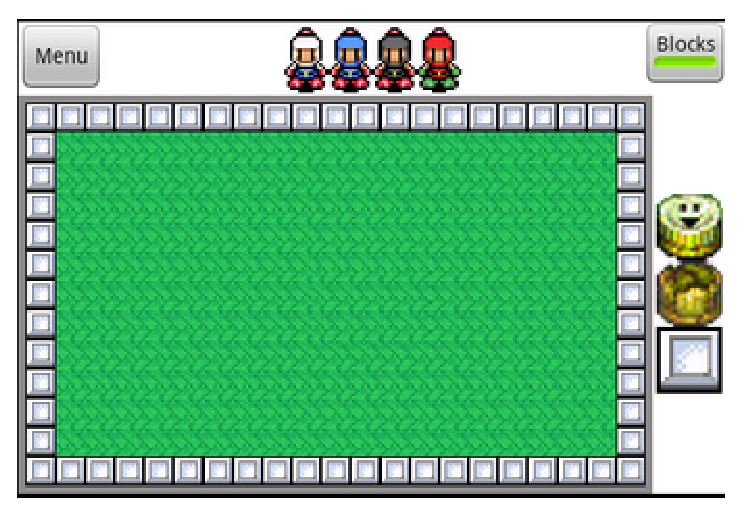
\includegraphics[scale=0.7]{Manuel/Img/11.eps}
		\caption{Edition de map}
	\end{figure}
	
	\paragraph{Enregistrement map\\}
	Une fois votre carte achevée ou non, vous pouvez accéder au menu d'option
	via le bouton Menu \textcolor{orange}{\textbf{1}} . Ce dernier vous propose
	alors de retourner sur l'éditeur \textcolor{orange}{\textbf{2}}, d'enregistrer votre
	carte et quitter \textcolor{orange}{\textbf{3}}, de remettre à zéro votre carte
	\textcolor{orange}{\textbf{4}}, et enfin quitter sans enregistrer
	\textcolor{orange}{\textbf{5}}. 
	
	\begin{figure}[h]
	\centering
		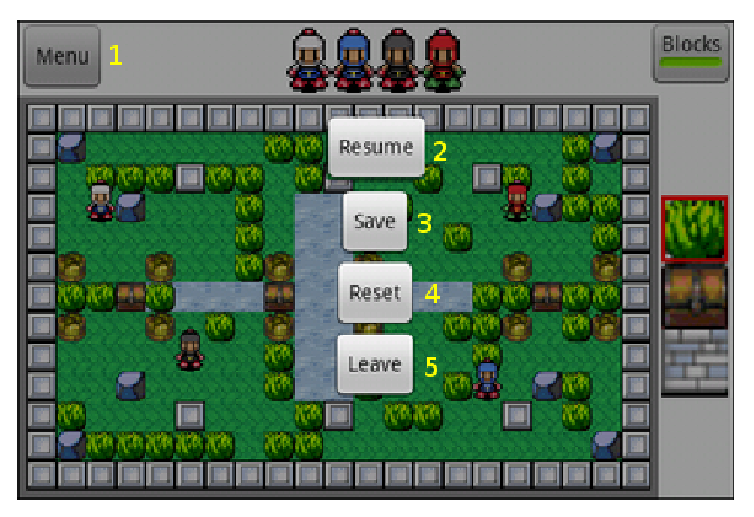
\includegraphics[scale=0.7]{Manuel/Img/13.eps}
		\caption{Option éditeur}
	\end{figure}
	
	\paragraph{Charger map\\}
	Après avoir enregistré une carte que vous ou un autre compte local aurait crée,
	il vous sera possible de l'éditer et de l'enregistrer et ce en la choisissant
	\textcolor{blue}{\textbf{1}} parmi toutes les cartes crées et de valider
	\textcolor{blue}{\textbf{2}}. \begin{figure}[h]
	\centering
		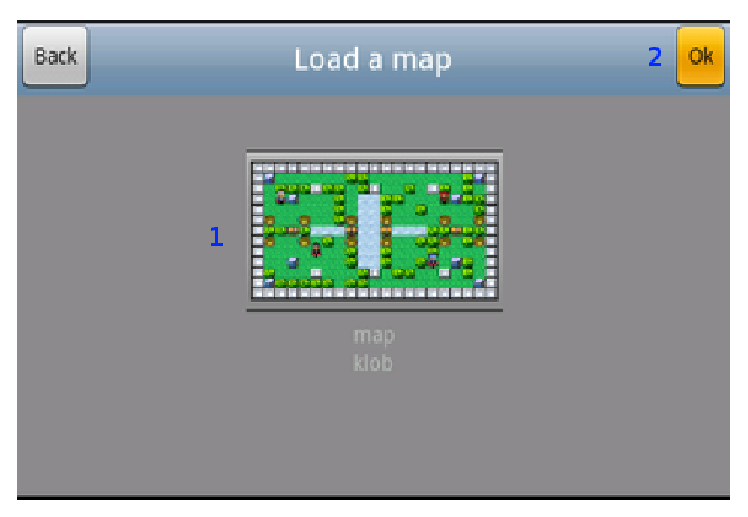
\includegraphics[scale=0.7]{Manuel/Img/14.eps}
		\caption{Charger une map préexistante}
	\end{figure}
	

\subsection{Options \textcolor{red}{4}}
	Le menu d'options est à votre disposition pour régler vos paramètre systèmes
	mais aussi profils d'utilisateur local et multiplayer.
	
	\paragraph{Réglage sytème\\}
	Ce type de réglage a été conçu pour ajuster le son
	\textcolor{blue}{\textbf{1}} à votre convenance mais aussi choisir la langue
	\textcolor{blue}{\textbf{2}} utilisée dans votre jeu. Sont à votre disposition
	le français mais aussi l'anglais.
	
	\begin{figure}[h]
	\centering
		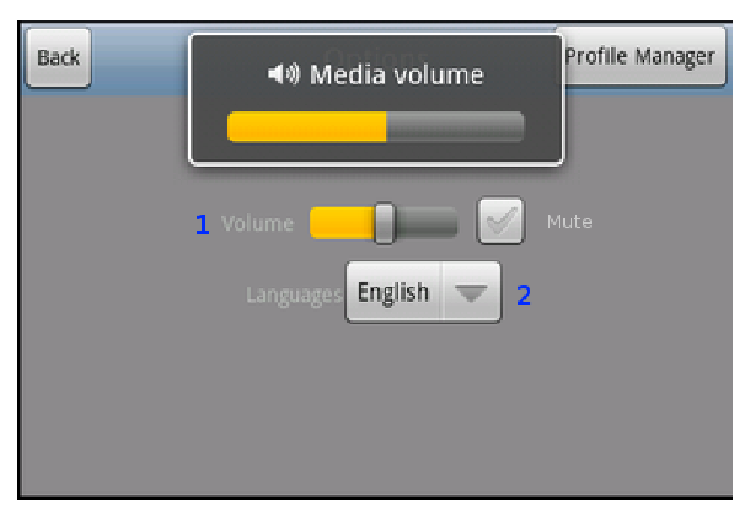
\includegraphics[scale=0.7]{Manuel/Img/4.eps}
		\caption{Charger une map préexistante}
	\end{figure}
	
	\subsubsection{Gestionnaire profil}
		Dans ce menu vous avez accès à l'édition de vos profils locaux et
		multijoueurs. Une fois vos modifications accomplies n'oubliez pas de les
		valider en cliquant sur le bouton Ok situé en haut à droite de votre fenêtre.
		\paragraph{Local\\}
		Il vous est ici possible de changer le pseudonyme \textcolor{blue}{\textbf{1}}
		de votre compte local en cour, mais aussi de choisir la couleur de votre
		personnage \textcolor{blue}{\textbf{2}} , toujours pour les parties locales.
		\begin{figure}[h]
			\centering
				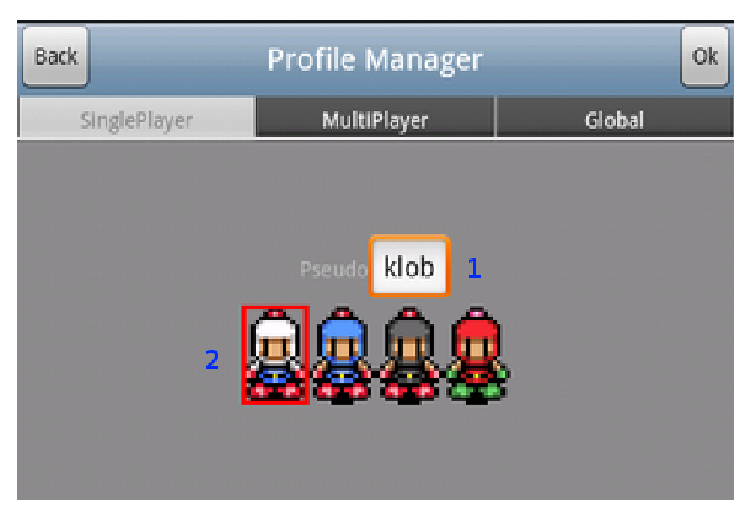
\includegraphics[scale=0.7]{Manuel/Img/5.eps}
				\caption{Gestion profil local}
			\end{figure}
		
		\paragraph{Multijoueur\\}
		Une fois un compte multijoueur crée sur le serveur, cet onglet vous donnera la
		possiblité d'éditer \textcolor{blue}{\textbf{1}} userName et password mais
		aussi de changer de compte multijoueur \textcolor{blue}{\textbf{2}}. Les
		paramètres d'accès comme la connexion automatique
		\textcolor{blue}{\textbf{3}} ou la sauvegarde du mot de passe
		\textcolor{blue}{\textbf{4}} sont ici configurables dès lors que le couple
		userName/password sera renseigné et valide.
		
		\begin{figure}[h]
			\centering
				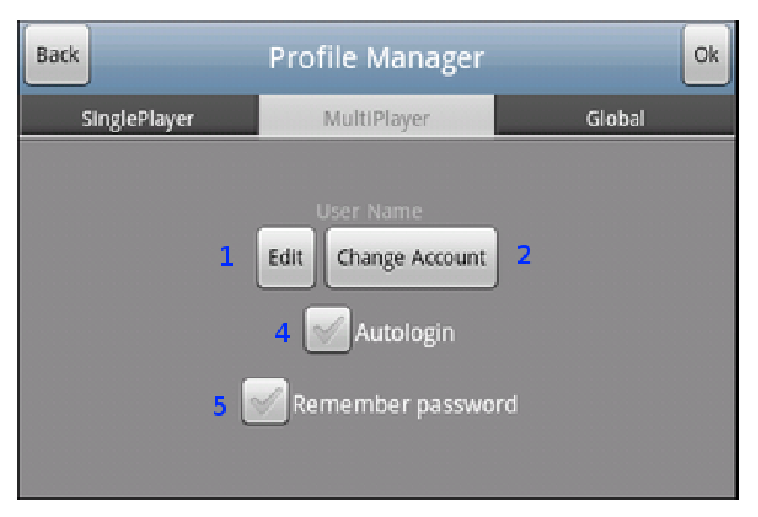
\includegraphics[scale=0.7]{Manuel/Img/6.eps}
				\caption{Gestion profil multijoueur}
			\end{figure}
		
		
		\paragraph{Général\\}
		Grace au menu déroulant \textcolor{blue}{\textbf{1}} vous pouvez fixer le
		côté de l'écran où sera positionné le menu de jeu, c'est à dire celui contenant le bouton de posage de bombes pendant une
		partie, suivant si l'on est gaucher ou droitier. 
		\begin{figure}[h]
			\centering
				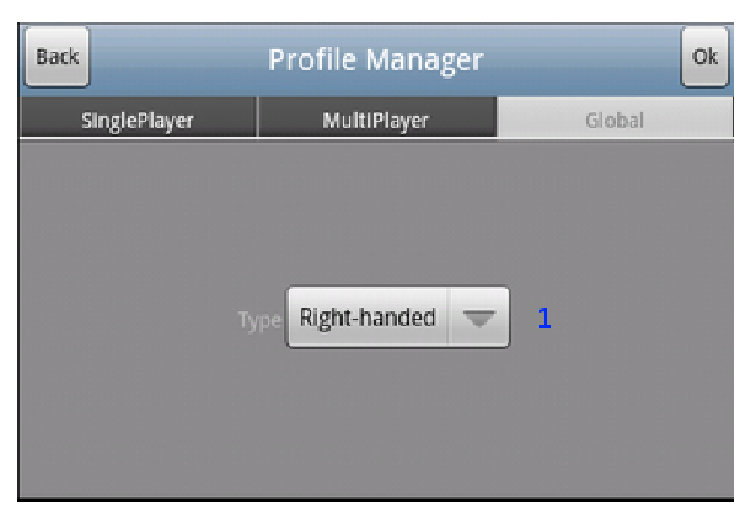
\includegraphics[scale=0.7]{Manuel/Img/7.eps}
				\caption{Général}
			\end{figure}
			
			
\paragraph{Choisir compte local \textcolor{red}{5}\\}
	Afin de permettre l'utilisation de l'application par plusieurs joueurs et donc
	comptes. Il vous est possible de les sélectionner grâce à une liste des comptes
	locaux. 
	\begin{figure}[h]
	\centering
		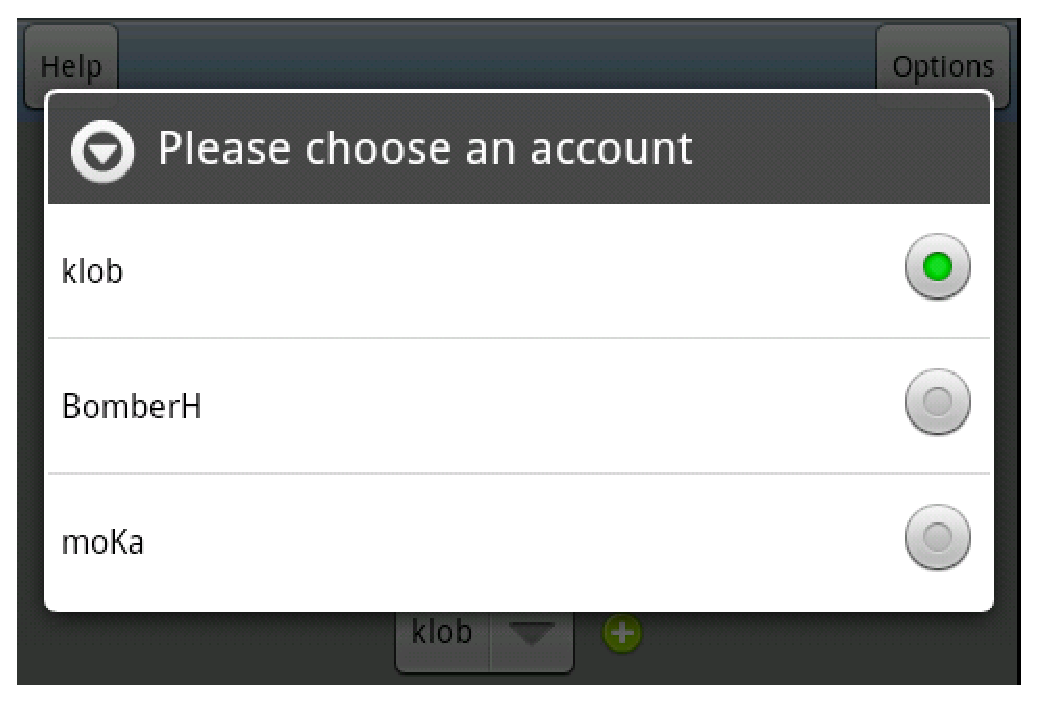
\includegraphics[scale=0.5]{Manuel/Img/8.eps}
		\caption{Choix compte local}
	\end{figure}

\paragraph{Ajouter compte local \textcolor{red}{6}\\}
	Il vous est demandé comme au premier lancement, de renseigner un pseudonyme 
	\textcolor{blue}{\textbf{1}}. Dans ce cas là une vérification que votre
	pseudonyme n'existe pas déjà serait faite. Une fois valide vous revenez sur le menu d'accueil avec votre
	nouveau compte local sélectionné.
	\begin{figure}[h]
	\centering
		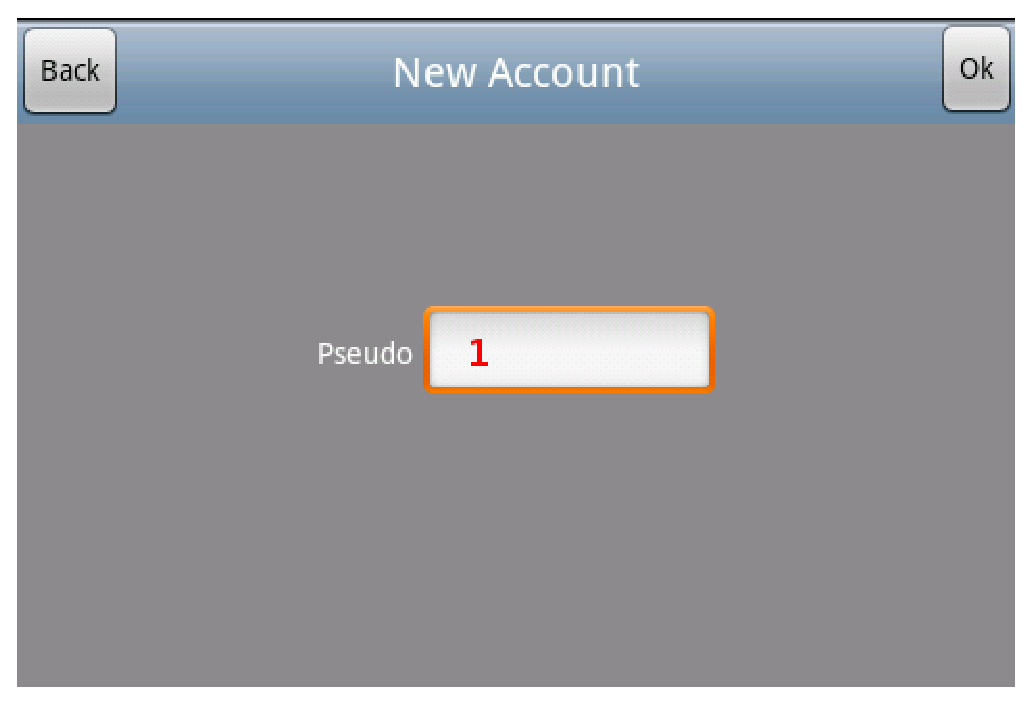
\includegraphics[scale=0.6]{Manuel/Img/9.eps}
		\caption{Ajoût nouveau compte local}
	\end{figure}
	
	
	TODO ludo

\section{Jeu}
	\input{Manuel/Parties/Jeu.tex}


\section{Editeur}
	\input{Manuel/Parties/Editeur.tex}

	

\chapter{Discussion}

	\section{Problèmes}
	Lors du developpement de notre projet nous avons été confronté à une multitude de problèmes. L'un des problèmes majeurs a été le manque de temps du à l'effectif de notre groupe de projet ainsi qu'à la quantité de travail que demandé la conception de ce projet. Ensuite plusieurs problèmes variés en fonction des plate-forme de developpent ont ralenti notre travail. De plus nous avons passé un peu trop de temps sur l'analyse malgres le fait que celle-ci nous ai permis de programmer aisément.

Le developpement mobile nous a aussi imposé de faible resource matérielle qui nous ont obligé à optimiser au maximum l'analyse et le developpement.


\subsection{Android}

\subsection{iOS}

Le premier problème rencontré avec le developpement d'une application sous IOS a été d'apprendre et maitriser le langage Objective-C qui nous été encore inconnu avant le developpement du projet. De plus la documentation et les informations sur ce langage étant seulement disponible en anglais nous a pas facilité la tache.
Un autre problème de l'Objective-C contrairement à JAVA est le manque d'un garbage collector \footnote{Un garbage collector(ramasse-miettes, ou récupérateur de mémoire ) est un sous-système informatique de gestion automatique de la mémoire. Il est responsable du recyclage de la mémoire préalablement allouée puis inutilisée.} Cela nous a obligé a géré la mémoire manuellement, chose que nous n'avions pas encore pris l'habitude de faire.
Ensuite le problème majeur est que pour tester une application IOS, il est obligatoire de posséder un compte \textit{IOS Developper Program} qui est payant et qui permet ensuite de mettre l'application à tester sur le téléphone. Car à cause de cela, il a été impossible de tester le gameplay de l'application IPhone.

	
		
\section{Améliorations}
	\subsection{Jeu}

Le developpement de ce type de jeu permet d'ajouter un grand nombres d'améliorations. Notament la gestion des bonus et des malus qui rendent le jeu beaucoup plus amusant et qui est disponible en annexe. Il y a aussi la gestion de différents types de parties, comme: la capture de drapeau,  les parties en équipe, etc. Nous aurions aussi pu ajouter un mode histoire pour les plus gourmands et pour rendre le jeu plus attractif. Puis une des améliorations les plus importantes, est l'ajout du mode multijoueur en WI-FI au niveau national (puis international ?) car ce dernier n'existe pas encore sur mobile et aurait très bien pu révolutionner le jeu bomberman sur mobile.


\subsection{Serveur}
	\begin{itemize}
		\item{Pooling}
		\item{Session}
	\end{itemize}

	
			
\chapter{Conclusion}

	L’application que nous avons réalisée est fonctionnelle et respecte les contraintes de fonctionnalités minimales imposées. Malheureusement nous n'avons pas eu le temps de developper le mode mutlijoueur  qui aurait été très enrichissant. Mais nous avons quand même implémenté la partie réseau qui  nous permettra dans un futur proche de pouvoir continuer à developper ce dernier dans le but de partager notre application sur l'AppleStore et l'AndroidMarket.

Toutes les fonctionnalités implémentées fonctionnent parfaitement malgres que durant le développement et les tests que nous avons réalisé, nous avons décelé quelques bogues minimes qui ont été corrigés au jour d’aujourd’hui.

Les langages que nous avons utilisés nous ont permis d'étoffer notre maitrise de la programmation objet et de découvrir le developpement mobile.
L'analyse du projet quand à elle s’est avéré suffisante et efficace car l’application fonctionne et que l’implémentation d’une multitude de fonctionnalités est envisageable.\\

Nous avons du développer cette application à quatre. Cela a été un handicap car nous disposions d’un temps limité et que le développement de deux applications comme celle-ci demande une vraie équipe de projet composée de plusieurs membres. Heureusement, gâce à notre organisation, à la bonne entente et la bonne communication au sein du groupe, nous avons pu travailler de manière efficace. Mais cela nous a aussi permis de partager nous connaissances et de nous entraider tout au long de ce projet.

\end{document}
